\documentclass[UTF8,fontset=fandol,zihao=-4]{ctexart}
\usepackage[a4paper,margin=25mm]{geometry}
\usepackage{amsmath,amssymb,amsthm}
\numberwithin{equation}{section}
\usepackage{graphicx,booktabs,tabularx,siunitx,placeins}
\renewcommand{\tabularxcolumn}[1]{>{\raggedright\arraybackslash}p{#1}}
\usepackage[font=small,labelfont=bf]{caption}
\usepackage[numbers,sort&compress]{natbib}
\usepackage{xurl}
\usepackage[hidelinks]{hyperref}
\setlength{\emergencystretch}{2em}
\setlength{\tabcolsep}{5pt}
\renewcommand{\arraystretch}{1.15}
\setcounter{topnumber}{3}
\renewcommand{\topfraction}{.85}
\renewcommand{\textfraction}{.10}
\renewcommand{\floatpagefraction}{.70}
\raggedbottom
\bibliographystyle{unsrtnat}

\title{面向同精度不可压流计算的\\随机特征 Galerkin 方法：\\离散结构、GPU 算子与端到端性能归因}
\author{}
\date{}
\hypersetup{pdftitle={面向同精度不可压流计算的随机特征 Galerkin 方法：离散结构、GPU 算子与端到端性能归因},pdflang={zh-CN}}
\begin{document}
\maketitle
\begin{abstract}
本文研究固定随机特征 Galerkin 不可压流求解器的数学适配与底层实现，区分试验空间、时间策略、单次算子成本及运行时开销对性能的贡献。对无反射约束的二维有限圆环流动，给出边界相容的随机特征构造、加权秩截断和含独立均值块的弱离散。推导带边界提升的一次变步 SBDF2 桥接及局部一致性，并在同一角模中构造共同相位坐标，证明几何锚点对指定条件数上界的极小极大性质。工程部分明确 FP64 FFT 打包与共享内存融合、warp 探针归约、C 语言径向内核以及准备和编译缓存的作用。\(Re=100\)、\(T=72\) 下，39 个配置在两种缓存政策下的 78 条 GPU 轨迹均满足速度与涡量 \(0.5\%\) 门槛；分段策略减少真实非线性求值 \(11.11\%\) 和 \(9.36\%\)。融合 FFT 缩短短程推进时间 \(9\%\)--\(17\%\)，却使首次完整求解增加 \(23\%\)--\(69\%\)。新增独立算子验证还显示，实场打包对强弱通道比例敏感，需单独检查弱通道误差。Legendre 降秩对照亦能通过精度门槛，最终隔离计时未被接受，因此尚不能建立随机特征相对同等优化传统 CFD 的整体速度优势。本文提供可复核的离散推导、源码级成本解释与有明确范围的正负结果；局部一致性、变换坐标条件数和数值资格均不被解释为完整非线性稳定性或普适性能保证。

\par\smallskip
\noindent\textbf{关键词}\quad 随机特征方法，Navier--Stokes 方程，Galerkin 方法，变步长 SBDF2，GPU 算子，性能归因
\end{abstract}
\section{引言}
\label{sec:introduction}

以神经特征构造数值试验空间，为偏微分方程提供了多项式基之外的选择。然而，一个流动求解器同时包含函数表示、空间投影、时间积分、线性代数、非线性变换与运行时管理。将这些部分一起替换之后获得的加速，不能自动归于随机特征。本研究针对这一归因问题，考察固定随机特征 Galerkin 方法在二维非稳态不可压流中的数值可行性，以及其数学结构如何转化为可测量的计算收益。

非稳态尾迹使比较尤其困难。速度是流函数的一阶导数，涡量涉及二阶导数；速度误差较小的近似，仍可能给出较差的涡量。交替涡脱落还会积累相位误差。如果允许每条轨迹独立平移时间，图像可能相似而原始初边值问题的解已不同。另一方面，在小型 GPU 问题上，一次算子调用只有几十微秒，设备编译、模块装载、FFT 计划及上下文初始化却可能占据可观的完整求解时间。因此，本文把共同物理精度、原始时间坐标以及端到端成本同时作为比较条件。

研究对象是有限圆环内、无反射约束的 \(Re=100\) 流动，积分至 \(T=72\)。径向分别采用固定随机三角特征、确定性 Legendre 特征与四阶空间有限差分；角向保留完整实 Fourier 表示。三个方法族使用一致的物理问题及二阶时间积分。Legendre--Galerkin 本身就是传统 CFD 对照，不应因其使用谱基而被排除。本文并不将固定特征 Galerkin 求解器等同于通过优化器训练整段轨迹的 PINN。

本文围绕以下三个问题组织方法与证据：第一，在保留速度与涡量精度时，分段时间步和较小试验空间能够减少多少实际工作？第二，共同相位坐标、FFT 融合和并行观测分别改变哪些计算环节，代数简化是否仍被实现中的其他成本抵消？第三，在相同精度、初始化政策和计时边界下，当前证据是否足以支持相对强确定性对照的整体速度优势？这三个问题分别需要离散分析、算子测试和完整隔离实验，不能由单一加速比回答。

\begin{table}[!htbp]
\centering\small
\caption{本文工作的归属与可支持的结论。数学适配不等于全新基本算法，局部实现收益不等于完整求解优势。}
\label{tab:contribution-map}
\begin{tabularx}{\linewidth}{@{}>{\raggedright\arraybackslash}p{.20\linewidth}XXX@{}}
\toprule
工作 & 类别 & 已有证据 & 结论边界 \\
\midrule
边界提升与一次变步桥接 & 数值方法适配 & 局部一致性推导及整轨迹资格 & 无完整 NS 无条件稳定性定理 \\
共同相位坐标与锚点 & 线性代数分析 & 同角模代数恒等式及上界 & 上界最优不等于实测耗时最优 \\
径向保留空间与 Legendre 对照 & 离散设计与验证 & 五个固定种子及确定性降秩对照 & 无随机特征普适优势证明 \\
融合 FFT、warp 观测、C 内核 & 底层算子工程 & 源码、局部与短程验证 & 不属于第三方 FFT 库内部补丁 \\
准备复用、缓存与启动路径 & 运行工程 & 分阶段记录与缓存等价性 & 最终隔离排名尚未建立 \\
\bottomrule
\end{tabularx}
\end{table}

本文的主要结果是可复核的工作量减少和性能归因，而非普遍速度胜出。两档时间策略将真实非线性求值减少约 \(11.11\%\) 和 \(9.36\%\)；最终 39 个配置在两种缓存政策下产生的 78 条 GPU 轨迹全部通过登记的数值门槛。专用融合 FFT 在固定状态和短程推进中有效，但首次完整求解变慢。最终完整隔离批次未满足接受条件，因此结果部分不据其残余记录生成方法排名。这一边界决定了本文应被理解为数值计算与应用高性能计算研究，现有理论和实验尚不足以构成一般收敛理论或普适优于传统 CFD 的论断。

补充的两因素消融进一步检验随机性的必要性：固定频率中点且保留解析层函数时，两档配置仍通过共同场误差门槛；删除非零模解析层函数则使本次12个配置均不合格，但同时降低了保留秩。本文因此把结论限定为当前富集空间的有效性，不将其自动归因于随机抽样。新增径向/模态误差分解及延后换步对照见第~\ref{sec:review-experiments}节，非可分几何下丢失的代数结构见第~\ref{sec:geometry-scope}节。

\section{相关工作与研究定位}
\label{sec:related-work}

\subsection{随机特征、投影求解与训练型方法}

随机特征方法通过固定非线性特征并确定组合系数求解 PDE\cite{r1}。局部极限学习机将固定隐藏层与区域分解结合\cite{r2}，随机神经网络 Petrov--Galerkin 方法已用于弹性及 Navier--Stokes 方程\cite{r3}。高精度 RFM、随机预条件和正交特征学习分别讨论误差、病态性及表示质量\cite{r4,r5,r6}。这些工作意味着，随机基与 Galerkin 的结合、预条件或正交化均不能单独作为本文的新颖性主张。

时间依赖 RFM 还可使用时空特征、分片统一和整体或分块最小二乘求解\cite{r15}。本文采用另一条实现路径：仅径向试验空间使用固定随机特征，角向使用 Fourier，时间用逐步 IMEX 积分。它没有学习时间特征，也没有沿整条轨迹反复最小化残差。因而针对时空最小二乘块传递的理论，不能未经推导套用于这里的 SBDF2 演化；其相反方向的性能结论也不能直接移植。

PINN 通过自动微分构造方程残差并训练网络参数\cite{r7}。因果训练调整演化问题的训练次序，PirateNets 用自适应残差结构改善深层 PINN 的训练\cite{r8,r16}。与这些方法比较时，应将训练、重启、采样、预测及导数重构按用途计入成本。已有论文中的误差和时间若采用不同几何、边界、终止时间或硬件，不能拼入本文的同精度表。当前结果没有这类同问题、同门槛的完整训练型对照，因此相关文献用于界定研究范围，不用于宣称本文更快。

\subsection{时间离散与线性代数结构}

IMEX 多步法及其变步推广已有系统研究\cite{r9,r12}。本文采用的二阶差分系数属于这一经典框架，新增分析针对当前离散质量、边界提升、历史通量包及一次步长切换的兼容关系。类似地，对称正定广义特征问题的白化与对角化是标准线性代数工具\cite{r10}。这里值得分析的是：同一角模多个时间相位能否共享坐标；如何界定锚点选择的作用；以及为何保持旧设备接口时，较少分解未必降低准备时间。

\subsection{GPU 融合与应用层性能}

FFT 去混叠、实场 Hermitian 结构和混合基算法都有成熟来源\cite{r11,r13}。cuFFTDx 已提供设备内 FFT、融合卷积及与 cuFFT 的比较示例\cite{r17}，warp 内交换和归约也属于 CUDA 标准编程机制\cite{r18}。本文的工程贡献是针对特定 FP64 多场通量布局实现并验证这些机制，保留强弱通道误差、启动负担和失败分支；不能把已有融合原理重新包装成新的 FFT 算法。

高层语言可以组织高性能流动求解，而计算密集部分由编译后的数值库或专用内核执行\cite{r14}。因此，本文按数据移动、同步、矩阵布局和生命周期讨论瓶颈。是否采用 C、CUDA 或其他宿主语言，应由所占成本和可减少的工作决定。相同原则也适用于开源贡献：本项目重写的是应用侧算子，当前没有修改第三方库源码。向上游贡献一个可复用样例，需要独立正确性、等价库实现对照和可复现构建，而不能仅凭本项目中的局部加速提出库性能修复。

\section{流动模型与固定试验空间}
\label{sec:governing-equations}
\label{sec:space-discretization}

\subsection{受驱动的有限圆环问题}

考虑二维不可压 Navier--Stokes 方程
\begin{equation}
 \partial_t\boldsymbol u+(\boldsymbol u\cdot\nabla)\boldsymbol u
 =-\nabla p+\nu\Delta\boldsymbol u,\qquad
 \nabla\cdot\boldsymbol u=0,\qquad
 \Omega=\{(r,\theta):a<r<R\}.
 \label{eq:ns}
\end{equation}
以圆柱直径和最终纵向来流速度为长度与速度尺度，取内半径 \(a=0.5\)、外半径 \(R=6\)、运动黏度 \(\nu=0.01\)，因此 \(Re=100\)，终止时间为 \(T=72\)。引入对数径向坐标 \(s=\log(r/a)\)，记 \(L=\log(R/a)\)、\(z=s/L\)，面积元为 \(r^2\,ds\,d\theta\)。

非零角向模态采用流函数表示：
\begin{equation}
 u_r=\frac{\psi_\theta}{r},\qquad
 u_\theta=-\frac{\psi_s}{r},\qquad
 \omega=-\frac{\psi_{ss}+\psi_{\theta\theta}}{r^2}.
 \label{eq:kinematics}
\end{equation}
角向均值则以独立的实切向速度 \(v(s,t)\) 推进，其径向速度为零、涡量为 \((v+v_s)/r\)。每个保留非零模态的正弦与余弦分量均参与演化，不施加反射对称或零环量约束。非零模态通过取旋度消去压力，独立的均值切向动量方程提供剩余的速度自由度。

流动从静止启动，驱动为
\begin{equation}
 U(t)=1-e^{-(t/0.8)^3},\qquad
 V(t)=\begin{cases}
 0.12\sin^4[\pi(t-4)/8],&4<t<12,\\
 0,&\text{其他时刻}.
 \end{cases}
 \label{eq:driving}
\end{equation}
有限时长的横向脉冲用于打破反射对称。内壁满足 \(\psi=\psi_s=0\)。外圆非零模态采用
\begin{equation}
 \psi(L,\theta,t)=R[U(t)\sin\theta-V(t)\cos\theta],\qquad
 \omega(L,\theta,t)=0.
 \label{eq:outer-boundary}
\end{equation}
均值块满足 \(v(0,t)=0\)、\(v_s(L,t)+v(L,t)=0\)。外边界并非完整速度 Dirichlet 条件，而是本有限域问题的组成部分，不能将其视为无限外域圆柱流动的精确透射边界。

给定边界数据由提升函数表示：
\begin{equation}
 \psi_\ell=\ell(s)[U(t)\sin\theta-V(t)\cos\theta],\qquad
 \ell(s)=R[(1-\beta)z^2+\beta z^3],\quad
 \beta=\frac{L^2-2}{4}.
 \label{eq:lifting}
\end{equation}
它满足 \(\ell(0)=\ell_s(0)=0\)、\(\ell(L)=R\)、\(\ell_{ss}(L)=R\)，最后一个恒等式保证 \(k=1\) 提升在外圆处的涡量为零。采用实场 Fourier 约定 \(f=c_0+2\operatorname{Re}\sum_{k=1}^{K}c_ke^{ik\theta}\) 时，复提升幅值为 \(g(t)=-(V(t)+iU(t))/2\)。物理重构、非线性投影和误差评价沿用同一约定，共轭负模完整表示实场。

有限外半径构成实质性限制。归档的外域敏感性诊断将 \(R\) 从6增至8后，共同 \(r\le4\) 区域的未对齐最大涡量差约为50.39\%，脱落频率亦有变化。因此，后文精度门槛针对指定的 \(R=6\) 问题；外域截断误差和离散误差不能互相替代。

\subsection{随机与确定性的径向试验函数}

对非零角向模态作展开
\begin{equation}
 \psi_k(s,t)=\sum_{j=1}^{d}F_j(s)x_{jk}(t)
                  +\delta_{k1}g(t)\ell(s),\qquad 1\le k\le K.
 \label{eq:trial-expansion}
\end{equation}
所有 \(F_j\) 均在时间积分前固定。RFM 在此指随机选择径向特征空间，再以确定性的 Galerkin 方程推进系数，不包含沿轨迹训练网络权重的过程\cite{r1,r2,r3}。

对奇数输入规模 \(m=2p+1\)，原始随机特征由常数和 \(p\) 对正弦、余弦组成：
\begin{equation}
 \begin{gathered}
 b_j=\frac{62}{p}(j+\xi_j),\qquad
 \xi_j\sim\operatorname{Uniform}(0.2,0.8),\qquad j=0,\ldots,p-1,\\
 q_{j,0}(z)=\cos[b_j(z-\tfrac12)],\qquad
 q_{j,1}(z)=\sin[b_j(z-\tfrac12)].
 \end{gathered}
 \label{eq:random-features}
\end{equation}
随机抽样使用固定的 \texttt{NumPy default\_rng(seed)}，登记种子为7331、7687、8011、8353、9041。Legendre 对照将原始特征换为 \(P_j(2z-1)\)、\(j=0,\ldots,m-1\)，并沿用相同边界变换、富集、求积和时间离散。本文报告的配置不使用径向坐标扭曲。

边界条件通过解析变换施加。对原始函数 \(q\)，令 \(\chi(z)=16z^2(1-z)\)、\(b(z)=z^2(1-z)^2/2\)，定义
\begin{equation}
 \mathcal Bq(z)=\chi(z)q(z)
       -b(z)\left.\frac{d^2(\chi q)}{dz^2}\right|_{z=1}.
 \label{eq:boundary-transform}
\end{equation}
因为 \(b(0)=b'(0)=b(1)=0\)、\(b''(1)=1\)，所得函数满足 \(F(0)=F_s(0)=F(L)=F_{ss}(L)=0\)。故对每个 \(k\)，齐次模态同时满足圆柱处无滑移和外圆零涡量条件。式~\eqref{eq:boundary-transform}中的导数针对 \(z\)；换算为 \(s\) 导数时必须计入 \(L^{-1}\) 与 \(L^{-2}\)。

两种试验族均加入相同的六个解析外侧边界层函数。记 \(\delta=L-s\)，则
\begin{equation}
 E_\gamma(s)=z^2\left[\delta+
       \left(\gamma+\frac{2}{L}\right)\delta^2\right]e^{-\gamma\delta},
 \qquad \gamma\in\{16,36,80,165,340,660\}.
 \label{eq:layer-features}
\end{equation}
在 \(\delta=0\) 处，其 Taylor 展开的常数项和二次项均为零，因而具有相同的外边界齐次条件；\(z^2\) 因子提供内壁条件。这些函数用于解析本有限域边界条件产生的外侧薄层，不属于随机特征学习出的结构。

均值块在两种试验族中均采用确定性多项式空间。原始函数为 \(z[(L+2)-(L+1)z]\) 及 \(z(1-z)^2P_j(2z-1)\)，其中 \(j=0,\ldots,m_0-2\)、\(m_0=24\)；富集为 \(z[1+(\gamma+1+1/L)\delta]e^{-\gamma\delta}\)。它们均满足均值边界条件。最终配置加入六个富集后保留30个均值函数，因此随机性只存在于非零模态的径向空间。

\subsection{求积、秩选择与模型规模的含义}

径向积分在 \([0,L-0.12]\)、\([L-0.12,L-0.018]\)、\([L-0.018,L]\) 三段采用正权 Gauss 求积。总节点数为 \(q\) 时，令 \(b_q=\max(8,\lfloor q/6\rfloor)\)，三段节点数分别为 \(q-2b_q,b_q,b_q\)。两个主要 Galerkin 配置分别使用44/11/11和52/12/12。由于随机三角函数及指数富集不是多项式，求积只近似连续弱式。下面的正性结论精确适用于求积定义的离散矩阵，并非径向求积误差估计。

记 \(\widetilde F,\widetilde D,\widetilde D_2\) 为全部经过边界修正和富集的原始函数在求积节点的值及前两阶 \(s\) 导数，\(W=\operatorname{diag}(w_i)\)。构造
\begin{equation}
 \mathcal A=\operatorname{diag}(\sqrt{w_i}/r_i)
       (\widetilde D_2-\widetilde F),\quad
 S=\operatorname{diag}(\|\mathcal A_{:j}\|_2),\quad
 \mathcal A S^{-1}=U\Sigma V^{\mathsf T}.
 \label{eq:feature-svd}
\end{equation}
原始列范数必须非零。保留满足 \(\sigma_j>10^{-10}\sigma_1\) 的奇异值，定义
\begin{equation}
 C=S^{-1}V_d\Sigma_d^{-1},\qquad
 F=\widetilde FC,\quad D=\widetilde DC,\quad D_2=\widetilde D_2C.
 \label{eq:feature-transform}
\end{equation}
这是针对离散微分算子的归一化和秩截断，并非普通点值内积中的正交化。精确算术下有 \(\operatorname{diag}(\sqrt{w_i}/r_i)(D_2-F)=U_d\)，从而 \(k=1\) 的耗散 Gram 矩阵归一为 \(\nu I\)。此恒等式解释已有构造的性质，不是新实测的优化，也不保证全部角模均有相同条件性。均值空间相应地归一化 \(\operatorname{diag}(\sqrt{w_i})(\widetilde V+\widetilde V_s)\)。

RFM37 等标签中的数字是原始随机特征数，不是未知量数。富集增加列，截断又可能删除列。若非零模态保留秩为 \(d\)，均值秩为 \(d_0\)，则实系数自由度为 \(2Kd+d_0\)，最终配置的 \(d_0=30\)。同秩比较和同精度比较回答不同问题。较小的 RFM 输入特征数不能证明其保留秩小于 Legendre 对照；比较不同实现时，种子和截断阈值也属于必须固定的模型身份。

\section{弱形式与时间离散算法}
\label{sec:numerical-method}

\subsection{非零模态的质量、耗散和非线性通量}

对上述速度场，不可压条件使涡量方程在对数径向坐标中写为守恒形式：
\begin{equation}
 r^2\partial_t\omega+\partial_s(r u_r\omega)
 +\partial_\theta(r u_\theta\omega)
 =\nu(\omega_{ss}+\omega_{\theta\theta}).
 \label{eq:vorticity-conservative}
\end{equation}
对第 \(k\) 个 Fourier 系数以齐次径向基函数测试。代入 \(r^2\omega_k=-(\psi_{k,ss}-k^2\psi_k)\)，对质量项分部积分一次，得到 \(\int(F_i'\psi_k'+k^2F_i\psi_k)\,ds\)。对黏性项分部积分两次，得到负的 Gram 形式。边界项因 \(F_i\) 在两端为零、\(F_i'(0)=0\) 和 \(\omega_k(L)=0\) 而消失。施加给定径向求积后，矩阵为
\begin{align}
 M_k&=D^{\mathsf T}WD+k^2F^{\mathsf T}WF,
 \label{eq:mass}\\
 K_k&=\nu(D_2-k^2F)^{\mathsf T}
        \operatorname{diag}(w_i/r_i^2)(D_2-k^2F).
 \label{eq:dissipation}
\end{align}
对任意实系数向量 \(x\)，有
\begin{equation}
 \begin{aligned}
 x^{\mathsf T}M_kx&=\|W^{1/2}Dx\|_2^2+k^2\|W^{1/2}Fx\|_2^2,\\
 x^{\mathsf T}K_kx&=\nu\|
 \operatorname{diag}(\sqrt{w_i}/r_i)(D_2-k^2F)x\|_2^2.
 \end{aligned}
 \label{eq:gram-positivity}
\end{equation}
因此两矩阵在精确算术下对称半正定。\(M_k\) 在保留空间上的正定性还要求加权点值和一阶导数样本叠置后具有满列秩。式~\eqref{eq:dissipation}的紧凑形式与归档代码采用的展开式在精确算术下等价，其正性不消除浮点相消、装配非对称或坐标变换病态。

令 \(a_k,b_k\) 分别为求积节点上 \(u_r\omega,u_\theta\omega\) 的 Fourier 系数。对两个输运项分别分部积分，得到
\begin{equation}
 f_k=D^{\mathsf T}\operatorname{diag}(w_i r_i)a_k
      -ikF^{\mathsf T}\operatorname{diag}(w_i r_i)b_k.
 \label{eq:weak-flux}
\end{equation}
乘积使用包含均值块和边界提升的完整速度，在物理角坐标上计算后投影回保留频带。线性系统虽可逐角模独立求解，非线性乘积仍耦合所有模态，因此将线性求解对角化不会消除非线性 FFT 工作量。

对 \(k=1\)，提升投影为
\begin{equation}
 \begin{aligned}
 M_\ell&=D^{\mathsf T}W\ell_s+F^{\mathsf T}W\ell,\\
 K_\ell&=\nu(D_2-F)^{\mathsf T}
       \operatorname{diag}(w_i/r_i^2)(\ell_{ss}-\ell).
 \end{aligned}
 \label{eq:lift-projections}
\end{equation}
其他非零模态没有直接提升项。省略角模下标，并允许相应提升向量为零，半离散系统可统一表示为
\begin{equation}
 m'(t)+Kx(t)+g(t)K_\ell=f(t),\qquad
 m(t)=Mx(t)+g(t)M_\ell.
 \label{eq:semidiscrete}
\end{equation}
被求导的是完整弱质量 \(m\)，若只使用 \(Mx\)，将遗漏边界加速度。多个独立提升可把 \(gM_\ell\)、\(gK_\ell\) 分别换为相应求和。

\subsection{均值块为何需要独立方程}

对切向动量作角向平均，得到
\begin{equation}
 \partial_t v=-\langle u_r\omega\rangle_\theta
       +\frac{\nu}{r^2}(v_{ss}-v).
 \label{eq:mean-equation}
\end{equation}
本小节以 \(V,V_s\) 表示均值基的节点值及导数矩阵，区别于式~\eqref{eq:driving}中的横向脉冲。均值矩阵和右端为
\begin{equation}
 \begin{aligned}
 M_0&=V^{\mathsf T}\operatorname{diag}(w_i r_i^2)V,\qquad
 K_0=\nu(V+V_s)^{\mathsf T}W(V+V_s),\\
 f_0&=-V^{\mathsf T}\operatorname{diag}(w_i r_i^2)a_0.
 \end{aligned}
 \label{eq:mean-matrices}
\end{equation}
检验耗散形式时，展开 \(\int(V+V_s)(v+v_s)\,ds\)，两个交叉项合为 \([Vv]_0^L\)。利用 \(v_s(L)=-v(L)\)、\(v(0)=0\)，这正是对 \(-\int V(v_{ss}-v)\,ds\) 分部积分产生的边界项。该块没有直接提升项，径向通量前的负号来自切向动量方程。直接在式~\eqref{eq:mass}--\eqref{eq:weak-flux}中令 \(k=0\) 会得到另一种表示，不是本实现采用的均值方程。

\subsection{恒步积分与一次桥接}
\label{sec:time-phase}

基线采用 SBDF2：扩散隐式处理，非线性弱通量以两点外推处理\cite{r9,r12}。隐式 Euler 起步后，恒定步长 \(h\) 的更新为
\begin{equation}
 \begin{aligned}
 (\tfrac32M+hK)x_{n+1}
 ={}&2m_n-\tfrac12m_{n-1}+h(2f_n-f_{n-1})\\
 &-g_{n+1}(\tfrac32M_\ell+hK_\ell).
 \end{aligned}
 \label{eq:uniform-sbdf}
\end{equation}
初始化使用静止初值和给定平滑来流。Euler 起步本身不构成二阶收敛证明，仍须结合初值问题和后续多步演化检查一致性；当前静止初态的显式非线性源为零。

优化时间策略在 \(t_0=8\) 之前采用恒定步长 \(H\)，之后改用较大的恒定步长 \(h\)。仅跨越接口的首个更新具有不等的相邻时间间隔。记 \(t_-=t_0-H\)、\(t_+=t_0+h\)、\(\rho=h/H>0\)，定义
\begin{equation}
 a_0=\frac{1+2\rho}{1+\rho},\qquad
 b_0=1+\rho,\qquad b_1=\frac{\rho^2}{1+\rho}.
 \label{eq:bridge-coefficients}
\end{equation}
桥接更新为
\begin{equation}
 \begin{aligned}
 (a_0M+hK)x_+={}&b_0m_0-b_1m_-+
 h[(1+\rho)f_0-\rho f_-]\\
 &-g_+(a_0M_\ell+hK_\ell).
 \end{aligned}
 \label{eq:bridge}
\end{equation}
本小节的 \(m_0,f_0\) 下标表示时刻 \(t_0\)，不表示角向均值。历史质量已含各自时刻的提升，未来提升仅减去一次。\(\rho=1\) 时，式~\eqref{eq:bridge}精确还原恒步式~\eqref{eq:uniform-sbdf}。

\paragraph{命题1：含提升桥接的局部一致性。}
设精确半离散解轨迹在桥接附近满足 \(m\in C^4\)、\(f\in C^3\)，且 \(\rho\) 属于 \((0,\infty)\) 的固定紧子集。令 \(\delta=\max(H,h)\)，则式~\eqref{eq:bridge}的导数型残差为 \(O(\delta^2)\)，乘步长后的方程残差为 \(O(h\delta^2)\)。

\paragraph{证明。}
对三个质量值作二次插值，在 \(t_+\) 求导，得到 \(Dm_+=(a_0m_+-b_0m_0+b_1m_-)/h\)。两份通量的线性外推在同一端点给出 \((1+\rho)f_0-\rho f_-\)。在 \(t_+\) 附近作 Taylor 展开，有
\begin{align}
 Dm_+-m'(t_+)
 &=-\frac{h(h+H)}{6}m'''(t_+)+O(\delta^3),
 \label{eq:bridge-derivative}\\
 (1+\rho)f_0-\rho f_- - f(t_+)
 &=-\frac{h(h+H)}{2}f''(t_+)+O(\delta^3).
 \label{eq:bridge-extrapolation}
\end{align}
将其代入式~\eqref{eq:semidiscrete}，扩散与提升均在 \(t_+\) 取值，合并残差即得结论。再代入 \(m_+=Mx_++g_+M_\ell\) 得到桥接更新式。\hfill\(\square\)

该命题仅为局部一致性，不是非线性 NS 的无条件稳定性或长期收敛证明。后者还需要正则性、起步、扰动传播和稳定性估计。有限时长脉冲仅分段光滑，上述 Taylor 论证局限于远离脉冲端点的 \(t=8\) 桥接邻域。对标量零方程 \(y'=0\)，桥接差分满足
\begin{equation}
 y_+-y_0=\frac{\rho^2}{1+2\rho}(y_0-y_-).
 \label{eq:zero-equation}
\end{equation}
两档登记步长比分别为 \(8/7\) 和 \(19/17\)，对应差分因子为 \(64/161\) 和 \(361/935\)，恒步段因子为 \(1/3\)。这说明指定时间网格上的齐次差分有界。显式输运和模态耦合没有出现在该检验中，因此它不提供完整流动的稳定性定理。

工作量减少来自时间策略，与基族无关。在 \(T=72\) 时，时间率于 \(t=8\) 从128改为112，将总步数由9216降至8192；从152改为136，将10944降至9920。初始非线性源恒为零，Euler 第一状态预先构造；重复核只在 $t_1,\ldots,t_{N_{\rm step}-1}$ 求值，终态不再评估。因此实际登记求值次数分别为 \(9215\to8191\) 和 \(10943\to9919\)。该计数不预测完整求解耗时，因为后者还包含额外相位准备和启动。

\subsection{固定空间准备的复用}

\paragraph{命题2：精确算术下的准备复用。}
固定几何、黏度、特征族、随机种子、富集、求积、提升、列缩放和奇异值阈值。若基变换在步长相关矩阵之前形成且与时间步长无关，则保留基、秩、\(M,K,M_\ell,K_\ell\) 及未预收缩的非线性测试算子可仅准备一次，在精确算术下不改变各相位的离散更新。

\paragraph{证明。}
式~\eqref{eq:feature-svd}--\eqref{eq:feature-transform}和式~\eqref{eq:mass}--\eqref{eq:mean-matrices}均不含时间步长。相位依赖仅通过 \(a_jM+h_jK\)、其分解或应用及步长加权右端进入。复用这些运算的相同输入，仍给出相同线性方程。\hfill\(\square\)

已有构造路径接受 \(A_{\rm eff}=(3/2)M+h_{\rm eff}K\)。对桥接取 \(c=(3/2)/a_0\)、\(h_{\rm eff}=ch\)，则
\begin{equation}
 A_{\rm eff}=c(a_0M+hK),\qquad
 A_{\rm eff}^{-1}(cb)=(a_0M+hK)^{-1}b.
 \label{eq:bridge-reuse}
\end{equation}
历史质量系数乘以 \(c\)，但已经含 \(h_{\rm eff}\) 的通量包不得重复乘该因子。原先预收缩的非线性历史依赖旧相位的逆矩阵，必须在接口处从原始通量谱重新映射；直接沿用旧收缩向量将改变算法。

精确算术等价不保证跨实现的逐位相同。归档在24组固定比较中验证了936项数组的字节一致，保留了原浮点表达式分组和计算环境。改变求和顺序、库、试验空间、提升或自适应策略后，须重新验证。共享准备减少重复空间工作，但仍保留相位分解、算子包、传输和执行图，因而不是一项独立的端到端计时结论。

\section{共同相位坐标与代数改良的边界}
\label{sec:phase-analysis}

\subsection{单一角模的同时同余变换}

固定一个角模，各相位矩阵写成 \(A_j=a_jM+h_jK\)，其中 \(a_j,h_j>0\)。前后恒步相位及桥接均具有这一形式。为避免与前段步长 \(H\) 混淆，将参考矩阵记为 \(H_*\)。假设 \(M,K\) 实对称半正定，且对正数 \(a_*,h_*\)，\(H_*=a_*M+h_*K\) 正定；等价地，\(M,K\) 没有共同非零零空间向量。广义对称正定特征问题的经典工具\cite{r10}给出如下表示。

\paragraph{命题3：共同相位坐标。}
存在实可逆矩阵 \(P\)，使 \(P^{\mathsf T}H_*P=I\)、\(P^{\mathsf T}MP=\operatorname{diag}(\lambda_i)\)。令 \(\theta_i=a_*\lambda_i\)，则
\begin{equation}
 \begin{gathered}
 0\le\theta_i\le1,\qquad
 P^{\mathsf T}A_jP=\operatorname{diag}(d_{ji}),\\
 d_{ji}=\frac{a_j}{a_*}\theta_i+
             \frac{h_j}{h_*}(1-\theta_i)>0.
 \end{gathered}
 \label{eq:phase}
\end{equation}

\paragraph{证明。}
对 \(H_*=LL^{\mathsf T}\) 作 Cholesky 分解。对称半正定矩阵 \(L^{-1}ML^{-\mathsf T}\) 存在正交特征基 \(Q\)。取 \(P=L^{-\mathsf T}Q\)，便得到 \(P^{\mathsf T}MP=\operatorname{diag}(\lambda_i)\)、\(P^{\mathsf T}H_*P=I\)。又因 \(h_*P^{\mathsf T}KP=I-a_*\operatorname{diag}(\lambda_i)\) 半正定，故 \(0\le a_*\lambda_i\le1\)。代入 \(A_j\) 的线性组合即得式~\eqref{eq:phase}，其中每个对角值都是两个正数的凸组合。\hfill\(\square\)

因此
\begin{equation}
 A_j^{-1}b=P\operatorname{diag}(d_{ji}^{-1})P^{\mathsf T}b.
 \label{eq:phase-inverse}
\end{equation}
这是同余变换，不要求原坐标中的矩阵两两对易。相同假设下，独立均值矩阵也适用。Euler 矩阵虽具有正系数并符合代数形式，但归档的共同相位原型沿用了原 Euler 初始化，并未对该相位独立验证晋升。

\subsection{最坏谱界的几何锚点}

令 \(r_j=h_j/a_j\)、\(\eta=h_*/a_*\)、\(r_{\min}=\min_jr_j\)、\(r_{\max}=\max_jr_j\)。从 \(d_{ji}\) 提出 \(a_j/a_*\) 后，剩余因子为 \(\theta_i+(r_j/\eta)(1-\theta_i)\)，位于1与 \(r_j/\eta\) 之间，因而
\begin{equation}
 \kappa_2(P^{\mathsf T}A_jP)
 \le B_j(\eta)=\max\{r_j/\eta,\eta/r_j\}.
 \label{eq:bound}
\end{equation}
对有限正相位集合，有
\begin{equation}
 \eta_* = \sqrt{r_{\min}r_{\max}},\qquad
 \min_{\eta>0}\max_jB_j(\eta)=\sqrt{r_{\max}/r_{\min}}.
 \label{eq:anchor}
\end{equation}
证明只需注意最坏上界为 \(\max\{r_{\max}/\eta,\eta/r_{\min}\}\)。两项的乘积恒为 \(r_{\max}/r_{\min}\)，其最大值在两项相等时最小，遂得式~\eqref{eq:anchor}。

上界与实际谱必须区分。如果 \(\theta_i\) 未接近区间两个端点，该界可能很松。几何锚点最小化的是这个界，未必最小化给定矩阵的实际最大条件数。同比缩放 \(a_*,h_*\) 不改变此界，却改变对角值大小，所以该规则不说明所有分母接近1；它也不改变原坐标的 \(\kappa_2(A_j)\)，不约束 \(P,P^{\mathsf T}\) 应用过程中的往返误差。

几何锚点结论完成了代数推导和独立审读，未进入计时候选。早期共同相位原型测得的准备开销不能归于这一未经计时的锚点选择。推导和原型均不构成随机特征逼近理论，也不构成时间积分稳定性定理。

\subsection{共同坐标为何不必然产生更快求解器}

跨角模有 \(M_k=M^{(0)}+k^2M^{(1)}\)、\(K_k=K^{(0)}+k^2K^{(1)}+k^4K^{(2)}\)。对 \(k^2\) 的多项式依赖不蕴含共同特征基。在固定白化度量中，一组实对称系数矩阵能够被同时正交对角化，当且仅当它们两两对易。归档测得的归一化交换子约为0.051--0.076，不支持以单个精确共同变换替代所有角模。

即使只考虑单一角模，设备端的数据接口仍决定收益。若设备需要预收缩稠密算子 \(A_j^{-1}B\)，其中 \(B\) 收集质量和非线性投影列，保持原接口仍须对每个相位形成 \(P\operatorname{diag}(d_j^{-1})P^{\mathsf T}B\)。对秩 \(d\)、与 \(q\) 成比例的投影宽度和 \(p_{\rm ph}\) 个相位，这需要一次 \(O(d^3)\) 特征分解及约 \(p_{\rm ph}+1\) 次 \(O(d^2q)\) 稠密乘法；直接路线则进行 \(p_{\rm ph}\) 次分解和各相位应用。共同表示仍须写出全部相位包。因此需要共同评估运算数、库吞吐、条件性和内存布局。

另一种设计可令时间系数始终保存在 \(P\) 坐标中，各相位仅作对角更新。但这同时要求对每个角模改写重构、提升、非线性投影和观测算子。现有完整轨迹证据没有验证该设计，它是一条具体工程方向，不能从式~\eqref{eq:phase-inverse}直接推断速度优势。

\subsection{区分逼近、积分与实现误差}

误差需要在四个层次上讨论：连续有限域解、求积定义的空间半离散解、其精确算术时间离散解，以及实际浮点执行解。相应区别外域误差、试验空间与求积误差、时间离散误差和实现误差。对于共同物理重构网格，使用同一绝对范数可通过三角不等式得到加性分解；相对误差则必须明确换算分母，不能直接相加以不同参考场为分母的两个百分比。

本文物理门槛是相对于两份高分辨数值参考的误差检查，实现门槛是同一离散方法的 GPU 与 CPU 差异。二者都不是对未知连续真解误差的严格上界。与此同时，较小速度误差不控制其空间导数；式~\eqref{eq:kinematics}中的涡量需要流函数二阶导数，因此涡量与近场门槛必须独立施加。

一个条件性扰动估计可解释为何算子残差小仍须检查轨迹。考虑同一离散步和相同提升的两次执行，系数差分别为 \(e_n,e_{n-1}\)，乘步长后的线性方程中出现加性残差 \(r_{n+1}\)。若非线性映射在包含两条轨迹的区域内满足 Lipschitz 常数 \(L_f\)，则对相容的系数范数有
\begin{equation}
 \begin{aligned}
 \|e_{n+1}\|\le\|A_n^{-1}\|\big[&
 (b_0\|M\|+h(1+\rho)L_f)\|e_n\|\\
 &+(b_1\|M\|+h\rho L_f)\|e_{n-1}\|
 +\|r_{n+1}\|\big].
 \end{aligned}
 \label{eq:perturbation-accounting}
\end{equation}
将两更新式相减，再使用范数和局部 Lipschitz 不等式即可证明。该式只是同一有限维离散格式的扰动记账，其常数可能很保守，并不建立一致的长期误差界。它说明单次 FFT 一致、小线性残差或良好的变换后条件数，都不能替代完整积分时域上的物理精度检查。

\section{底层算子与计算成本}
\label{sec:operators}

\subsection{保持离散不变的算子边界}

非线性算子的输入是径向重构之后的各物理场角向半谱，输出是径向投影或有限差分右端构造之前的通量半谱。明确这一边界后，替换核必须从同一组重构系数计算同一去混叠乘积。减少真实时间样本、改变求积，或把弱通量形式改为另一种离散对流形式，都会改变数值方法，必须另外验收，不能被算子融合隐含地带入。

令 \(q\) 为该阶段的径向行数，\(N\) 为角向变换长度，\(H_N=\lfloor N/2\rfloor+1\) 为半谱宽度。数据按场优先排列，场 \(c\)、径向行 \(i\)、非负模态 \(k\) 的线性地址为 \(((cq+i)H_N+k)\)，每项保存一对 FP64 实虚部。Galerkin 读入 \(u_r,u_\theta,\omega\) 三个平面，返回 \(u_r\omega,u_\theta\omega\) 两个通量平面。FD 读入四个平面，返回两项导数乘积之和的一个平面；径向度量因子沿用原重构与右端约定。FD 的独立均值强迫由外部提供，仍按原角模升序相加。两条路径均在覆盖当前通量前，将原始通量复制到规定的 SBDF2 历史缓冲。

基线依次调用一次批量 cuFFT 逆变换、一个乘积核及一次批量 cuFFT 正变换。一个批量调用包含多个场和径向行，cuFFT 内部也可能启动多个设备核\cite{r11}。因此，三个高层操作不等于三个单场变换，更不等于性能分析器观测到的三个 GPU 节点。Galerkin 每行需要三个实逆变换和两个实正变换；FD 需要四个逆变换和一个正变换。二者均保留五个逻辑场变换。本节优化改变它们的实现方式。

\begin{figure}[!htbp]
\centering
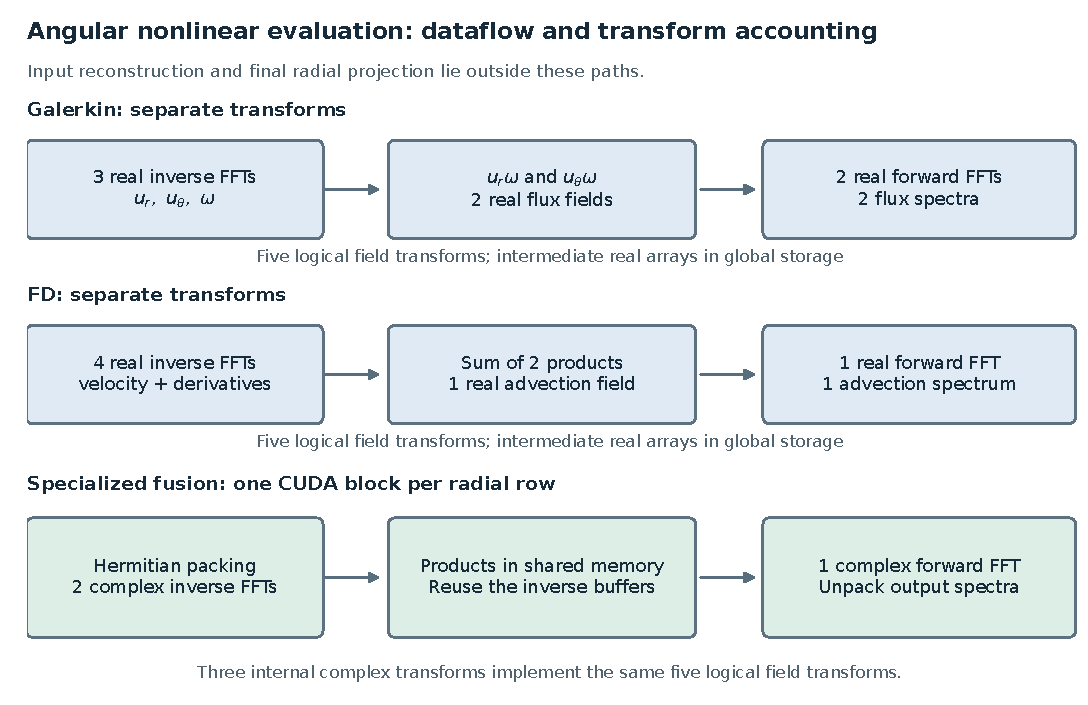
\includegraphics[width=\linewidth]{figures/nonlinear_pipeline.pdf}
\caption{非线性算子的替换边界。两种离散各自保留原有物理乘积。融合在共享内存中组织角向变换、点乘和打包；径向重构及投影位于图示替换范围之外。两种路径均保留五个逻辑场变换。}
\label{fig:operator-pipeline}
\end{figure}

\subsection{实场打包恒等式与归一化}

定义未归一化的正、逆离散 Fourier 变换为
\begin{equation}
\label{eq:op-dft}
(\mathcal F_N v)_k=\sum_{j=0}^{N-1}v_j e^{-2\pi\mathrm{i}jk/N},\qquad
(\mathcal B_N A)_j=\sum_{k=0}^{N-1}A_k e^{2\pi\mathrm{i}jk/N}.
\end{equation}
因此 \(\mathcal B_N\mathcal F_N=NI\)。CUDA 替换遵循 cuFFT 的符号及归一化约定\cite{r11}，不额外乘 \(1/N\)。求解器后续投影或 FD 右端已经包含相应尺度；若在两处同时归一化，即使单独的正逆变换测试看似正确，也会改变实际非线性方程。

对两个分别满足 Hermitian 对称的谱 \(A,B\)，由线性性可得
\begin{equation}
\label{eq:op-inverse-pack}
\mathcal B_N(A+\mathrm{i}B)=a+\mathrm{i}b,
\qquad a=\mathcal B_N A\in\mathbb R^N,\quad b=\mathcal B_N B\in\mathbb R^N.
\end{equation}
负模必须按 \(\overline{A_k}+\mathrm{i}\overline{B_k}\) 分别重建；若把整个打包正模共轭，则得到错误的 \(\overline{A_k}-\mathrm{i}\overline{B_k}\)。打包后的复谱通常不再满足 Hermitian 对称。零频和偶长度的 Nyquist 频率处，每个原实场谱的虚部须为零。

形成两个实乘积 \(g,h\) 后，令 \(Z=\mathcal F_N(g+\mathrm{i}h)\)，可恢复各自的谱：
\begin{equation}
\label{eq:op-forward-pack}
G_k=\frac{Z_k+\overline{Z_{-k}}}{2},\qquad
H_k=\frac{Z_k-\overline{Z_{-k}}}{2\mathrm{i}}.
\end{equation}
Galerkin 使用一次打包复逆变换重构两速度，一次逆变换重构涡量，一次打包复正变换恢复两个通量。FD 分别打包两速度和两导数，形成点积后作一次正变换。因此内部都执行三个复变换。这是实现层的计数恒等式，不能推出 \(5/3\) 的加速比：原 cuFFT 实变换已经利用 Hermitian 冗余，打包、置换、同步及额外指令均有成本。

保留带为 \(|k|\le K\) 时，二次乘积谱支撑至多为 \(2K\)。若别名进入保留模态，则存在非零整数 \(\ell\) 使 \(|k+\ell N|\le2K\)。而 \(|k+\ell N|\ge N-K\)，故严格条件 \(N>3K\) 排除了这一可能。这是经典的保留带去混叠论证\cite{r13}，并不表示乘积中不存在高于 \(K\) 的模态，也不能消除径向求积误差。替换核保持原角向填充长度和截断方式。

\subsection{线程映射、同步与访存}

每个径向行由一个128线程块处理，两块各含 \(N\) 个复双精度数的共享数组保存打包逆变换输入及物理场。专用长度及分解为 \(200=2^3 5^2\)、\(225=3^2 5^2\)、\(243=3^5\)，每块共享存储分别为6400、7200、7776字节。它们是明确实例化的长度，不是通用任意长度 FFT 服务。

设有序基数为 \(r_0,\ldots,r_{s-1}\)，将位置展开为混合进制数字 \(d_j\)，装载置换为
\begin{equation}
\label{eq:op-permutation}
p(i)=\sum_{j=0}^{s-1}d_j\frac{N}{\prod_{\ell=0}^{j}r_\ell},\qquad
i=\sum_{j=0}^{s-1}d_j\prod_{\ell=0}^{j-1}r_\ell.
\end{equation}
在前序基数积为 \(m\)、当前基数为 \(r\) 的阶段，各蝶形在乘旋转因子后合并间隔为 \(m\) 的位置。线程以128为跨度分配互不重叠的蝶形，相邻阶段之间执行全块屏障。这是经典混合基 FFT 构造；本项目的实现贡献在于它与当前算子边界及数据布局的结合，而非新的 FFT 分解。

完整执行顺序为：按置换装载两块打包逆变换平面，完成逆变换各阶段，各线程把一至两个物理乘积暂存寄存器，等待读取完成后覆盖第一块共享平面，执行正变换，拆包并写出半谱。寄存器暂存及覆盖前屏障必不可少，因为其他线程可能仍需读取原逆变换结果。即使全核只有一个线程块，省去该屏障仍会引入读写竞争。计入装载和覆盖屏障后，共有 \(2s+3\) 次全块同步，三种长度分别为13、11、13次。

原分离路径在全局内存中显式保存逆变换物理数组和正变换乘积数组。仅按这些命名数组的写入和读取计数，每次非线性评估名义消除 \(80Nq\) 字节访问：Galerkin 对应 \((3+3+2+2)Nq\) 个 double，FD 对应 \((4+4+1+1)Nq\) 个 double。这是这些实数组的源码级访问模型，并非设备总流量减少的上界；它未纳入缓存复用、编译器行为、库工作区，也不包含仍需保留的输入谱、输出谱及通量历史访问。因此它不是实测显存带宽数据，不能直接换算为速度增益。

融合同时增加共享存储、寄存器生命周期及单块工作量。径向行数较小时，线程块总数也可能不足以充分利用 GPU；消费级设备的 FP64 吞吐亦可能成为限制。由临时数组减少，不能直接判断最终算子受显存带宽、指令吞吐还是启动延迟限制。Roofline 或占用率结论需要本研究未采集的硬件计数器及受控测量。

\subsection{浮点边界与带保护的独立样例}

式~\eqref{eq:op-inverse-pack}--\eqref{eq:op-forward-pack}在精确算术下成立。浮点情况下，尺度为 \(A\) 的强通道可能向尺度为 \(B\) 的弱通道引入约 \(\epsilon A\) 量级的绝对扰动，对应相对尺度为 \(\epsilon A/B\)，还未计入变换常数和抵消。这是解释误差传播的尺度估计，并非该核的误差上界。它说明合并向量的相对误差很小，仍可能掩盖弱通道的相对误差；存在强抵消时，还需要按未抵消乘积大小缩放的绝对误差。

本次修订将原 CUDA 文件和既有 CPU 模型逐字提取，并新增不依赖求解器的验证入口及 NumPy、直接卷积参考。输入契约检查支持长度、连续 FP64 布局、实端点、零填充、有限数值及保留带宽。新增工程保护是：同一径向行内，若两个非零打包输入谱的最大模之比小于 \(10^{-8}\)，则默认拒绝执行。该阈值是保守的分派策略，不是保证相对精度的充分条件；严格为零的通道须采用绝对误差检查。真正的生产集成还需一个经验证的不打包后备路径，以及低成本获得尺度的方法；本样例没有宣称完成这些工作。冻结 NS 内核及其资格记录保持原状。

独立入口已在本机 GPU 完成36个固定态测试，覆盖三种长度、两种算子及每种算子六类输入。第六类在 Galerkin 中为一个速度通道严格为零，在 FD 中为两项相加抵消，因此两种算子合计使用七种不同标签。除独立 NumPy FFT 参考外，还使用不调用 FFT 的保留带多项式卷积参考，另验通量历史及 FD 均值缓冲奇偶位置。每输出通道的相对误差定义为跨径向行及半谱模态的无穷范数比 \(\max_{i,k}|Y_{ik}-Y^{\rm ref}_{ik}|/\max_{i,k}|Y^{\rm ref}_{ik}|\)，并非逐点相对误差。普通输入的各输出通道最大相对误差为 \(1.18\times10^{-15}\)。绝对误差诊断采用跨输出通道的统一尺度：对每行、每通量表达式，分别取各物理因子的最大模，将对应乘积相加并乘 \(N\)，最后在全部行和通道上取最大值。所有输入按此未抵消尺度缩放的最大绝对误差为 \(3.84\times10^{-16}\)；统一尺度可能掩盖弱通道误差，因此必须同时查看逐通道相对指标。将一个速度通道缩小到 \(10^{-10}\)，先确认保护拒绝，再显式放行作诊断后，单通道相对误差最大达到 \(4.98\times10^{-6}\)。这里采用向上取整的简写值，是新合成输入验证，不能替代原归档实测数字。本次提取未新增计时或 NS 轨迹，并以本地贡献候选的状态附于源码包。

\subsection{观测归约与 CPU 原生核}

探针算子计算六个加权和 \(p_j=w_j^\top x+\ell_j(t)\)。原实现让每个探针由一条线程串行处理；新实现为每个探针分配一个完整 warp，lane \(\ell\) 累加 \(\ell+32m\) 位置，再经五级 shuffle 归约合并\cite{r18}。一个192线程块覆盖全部六个探针。总算术工作仍与 frame 长度 \(L\) 线性相关，但每探针的串行深度由约 \(L\) 降为 \(\lceil L/32\rceil+5\)，这里没有把访存及指令成本视为零。快照复制、状态指针和推进前的同步均保留。求和次序改变会影响舍入，因此状态逐位不变与探针数值一致是两个独立检查。相应 Galerkin 与 FD 对照采用相同观测优化。

Python 驱动以下也有真实的项目内 C 实现。Galerkin 收缩核使角模成为连续内层维度，合并相同的预收缩质量与通量投影；FD 缓冲核应用已经装配好的窄径向模板，复用工作数组并就地形成物理乘积；另一个带状回代核用缓存的实 LAPACK 因子处理交错存储的复右端。FD 编译启用优化及 AVX2 支持，并关闭浮点乘加收缩，但编译选项本身不能证明 SIMD 利用率或加速。相应 CPU 变体仍调用 SciPy 的部分 FFT 或分解服务，并未修改其库源码和算法。

上述实现说明存在底层代码改动，但代码存在不等于完整求解已经通过隔离计时。同理，将 Python 调度语言整体替换为 Rust，不会直接减少设备 FFT 工作量、保留秩或编译核初始化成本。语言迁移应由实测宿主瓶颈或可复用接口需求驱动。本文区分循环和布局改动，以及导入、编译缓存、CUDA 图调度等运行时改动。

\subsection{完整成本、摊销条件与上游边界}

用于归因的成本分解为
\begin{equation}
\label{eq:cost}
\begin{aligned}
T_{\rm total}={}&T_{\rm start}+T_{\rm prepare}+N_{\rm nl}C_{\rm nl}\\
&+N_{\rm step}C_{\rm lin}+N_{\rm obs}C_{\rm obs}+T_{\rm finish}.
\end{aligned}
\end{equation}
各成本代表相位加权的有效量，并非假设每一步耗时相同。其中 \(C_{\rm lin}\) 不重复包含已经列出的非线性及观测开销。时间网格改动影响 \(N_{\rm nl},N_{\rm step}\)，融合影响 \(C_{\rm nl}\)，warp 归约影响 \(C_{\rm obs}\)，准备复用和缓存影响其他项。不能跨不相干测量直接相加收益，也不能重复计入同一成本。

若原固定执行中比例为 \(f\) 的部分获得局部加速比 \(s\)，理想整体界为 \([1-f+f/s]^{-1}\)。额外初始化成本会进一步缩小收益。更明确地，令 \(S_b,S_f\) 为基线和融合设置成本，\(B_b,B_f\) 为一份其余条件相同的重复工作成本；只有真实复用设置时，融合路径在 \(m\) 次重复后胜出才等价于
\begin{equation}
\label{eq:op-amortization}
m(B_b-B_f)>S_f-S_b.
\end{equation}
若每个新进程都重新构建或加载相关状态，设置就不是一次性成本，必须改写摊销模型。下一节的固定态事件测量及短轨迹结果说明，这一区分会改变结论。显式 PTX 缓存也不意味着驱动 JIT、模块加载、上下文、计划及进程启动成本全部消失。

完整求解时钟包含构造、编译或加载、传输、FFT 准备、图捕获、推进、观测、同步、下载和释放；新进程时钟再包含解释器启动、导入及规定监督开销。两者均不能由核事件替代。独立数值资格可以并发完成，但延迟比较须串行使用 GPU 并监测外部活动。CPU 总占用率不是同精度性能指标。

最后，源码审计识别到的是项目内应用核及库接口调用，没有发现已修改的 cuFFT、cuFFTDx、SciPy 或 LAPACK 借入源码。NVIDIA 已提供 FFT 融合与卷积示例，并包括 cuFFT 流水线及可选 LTO 回调的对照\cite{r17}。因此合理的上游方向是新增多场 FP64 的“逆变换、跨场乘积、正变换”示例，而非声称发明 FFT 融合或修复 cuFFT。提交仍需同等融合的 cuFFTDx 实现、批量 cuFFT 基线、相同精度和填充、首次及重复使用成本，以及脱离本机的干净构建。本地样例尚不满足这些性能与可移植性条件，也未建立新的许可证授权或贡献签署，尚未提交 PR\cite{r19}。

\section{实验设计与归因协议}
\label{sec:validation}

实验分别回答三个问题：离散方法能否达到指定物理精度，实现改动能否保持该离散的数值结果，以及合格实现能否缩短完整求解时间。三者需要不同对照。成功轨迹证明数值可行性，固定状态下更快的算子说明局部实现收益，完整配对计时才支持实际速度优势。以下同时报告成功与被淘汰的候选，并始终保留这些证据层次。

\subsection{算例、参考解与独立重构}

主要比较均采用 $a=0.5$、$R=6$、$\nu=0.01$、$T=72$ 的有限圆环。最终来流速度和圆柱直径均为1，故 $\mathrm{Re}=100$。横向脉冲在 $t=12$ 结束，观测持续到 $t=72$。计算没有反射约束；评分时不平移时间，也不对齐尾迹相位。对于给定初边值问题，累计相位偏差本身就是近似误差的一部分。

冻结的两份数值参考在归档中记为 \texttt{angular\_fine} 与 \texttt{time\_fine}，分别核查有限差分细化链中的角向与时间分辨率。细化链将径向区间数由384增至448、角向截断由128增至144、时间率由384增至512。它们是两份不同的数值参考，不是两套独立实现对连续真解给出的认证。晚期组合差为 $0.0290144\%$，小于候选门槛四分之一对应的经验参考预算 $0.125\%$；但它大于 $0.1\%$ 候选门槛所对应的 $0.025\%$ 预算。因此现有证据支撑本文采用的 $0.5\%$ 协议，不能自动升级为连续真解的严格误差界或更紧的验收标准。

所有方法先重构到同一物理网格再评分。对重构网格 $G$、检查时刻 $t$ 及其物理权重，定义
\begin{equation}
\label{eq:field-errors}
 E_u(G,t)=\frac{\|\boldsymbol u-\boldsymbol u_{\rm ref}\|_G}{\|\boldsymbol u_{\rm ref}\|_G},\qquad
 E_\omega(G,t)=\frac{\|\omega-\omega_{\rm ref}\|_G}{\|\omega_{\rm ref}\|_G}.
\end{equation}
积分测度为 $r^2\,ds\,d\theta$，速度范数共同计入两个极坐标分量。每个量分别检查全圆环及 $r\leq2.5$ 近场。三套重构网格分别使用123、129、144个径向点以及433、449、457个移位角向点，与求解器自身求积和FFT网格不同。具体构造及19个物理时刻见附录~\ref{sec:app-setup}。跨网格取最大值降低了结果对单一采样方式的依赖，但这些仍是有限个离散检查。

双参考物理误差在 $t=0.5$ 至72的19个时刻验收。分段方案在桥接后另存两个状态，用于实现一致性检查，因此归档区分19个物理时刻与21个实现检查状态。三个下游位置各保存横向速度和涡量，共六条探针历史，每条包含577个等间隔时刻，包括初始零值。GPU相对同离散CPU轨迹的场及完整探针序列误差门槛为 $10^{-5}$。尾迹检查还要求持续交替变号。合理的脱落频率和相似的图像均不能替代场误差验收。

\subsection{防止不同误差相消的保护条件}

分段方案的恒步控制保持同一空间、种子、几何和求积。令 $v$ 为恒步控制、$w$ 为分段候选、$z$ 为参考，并在同一加权范数下定义 $b=\|v-z\|_G/\|z\|_G$、$d=\|w-v\|_G/\|v\|_G$。则
\begin{equation}
\label{eq:triangle-guard}
 \frac{\|w-z\|_G}{\|z\|_G}
 \leq b+d\frac{\|v\|_G}{\|z\|_G}
 \leq b+(1+b)d.
\end{equation}
直接误差与 $b+(1+b)d$ 均须不超过0.005。直接使用 $b+d$ 会忽略两个相对误差的不同分母。保护量逐场、逐区域、逐网格、逐时刻、逐参考计算后再取最大值，防止时间调度误差恰好抵消恒步误差而造成表面合格。这是上述离散场之间的严格范数关系，不是对连续PDE真解的后验估计。

这项要求可以拒绝直接误差已合格的候选。高档Legendre34分段方案的直接场误差约为 $0.481690\%$，但三角保护达到 $0.509600\%$。其恒步方案仍合格且必须保留。当问题是达到共同精度的最小代价时，公平比较不要求各方法使用相同时间策略，更不能删除便宜的确定性替代方案。

\subsection{受控比较与计算环境}

表~\ref{tab:fairness}区分各项对照能够识别的贡献。同秩比较控制代数维度，不代表两族基在所有流动上具有相同逼近能力；最便宜合格配置的比较则允许秩与调度不同。两种问题都有意义，但结论必须分别标明。有限差分对照采用四阶径向空间差分及相同的二阶SBDF2时间离散；本文所称“四阶”不指时间格式。

\begin{table}[tbp]
\centering\small
\caption{比较矩阵及其能够识别的影响。物理比较均保持同一初边值问题与误差标准。}
\label{tab:fairness}
\begin{tabularx}{\linewidth}{@{}p{0.21\linewidth}XX@{}}
\toprule
对照 & 保持不变 & 允许变化及可解释量 \\
\midrule
RFM / Legendre同秩 & $K,q$、实际秩、调度、共同核与运行时政策 & 试验函数及其逼近误差 \\
同精度空间 & 参考、场和探针门槛、运行时政策 & 秩与合格调度；逐种子报告实际秩 \\
恒步 / 分段 & 同空间、种子、$K,q$及观测协议 & 时间调度与相应相位准备 \\
cuFFT / 融合核 & 输入、精度、保留频带、归一化及输出定义 & 变换实现与暂存方式 \\
串行 / warp观测 & 状态演化与探针权重 & 求和顺序及观测代价 \\
首次使用 / 缓存命中 & 求解器、产物、精度与新进程入口 & 显式编译产物的可用性 \\
Galerkin / FD & 物理问题、精度、观测与运行时政策 & 空间离散及其合格分辨率 \\
\bottomrule
\end{tabularx}
\end{table}

表~\ref{tab:hardware}列出归档实验环境。数值后端通过原生接口使用FP64 CUDA核和cuFFT，CPU参考及主机准备使用NumPy和SciPy。兼容性探针还验证过cuBLAS，但实际Galerkin推进使用项目自有投影核，不能把兼容性测试写成生产路径的cuBLAS加速。

\begin{table}[tbp]
\centering\small
\caption{归档Windows实验记录的环境。版本是实测条件，不表示当前推荐版本。}
\label{tab:hardware}
\begin{tabularx}{\linewidth}{@{}lX@{}}
\toprule
组件 & 记录值 \\
\midrule
CPU & AMD Ryzen 9 9955HX，16核、32逻辑处理器 \\
GPU & NVIDIA GeForce RTX 5060 Laptop GPU；计算能力12.0 \\
系统 / 驱动 & Windows 11，构建26200；NVIDIA 596.13，WDDM \\
科学计算环境 & Python 3.13.5；NumPy 2.2.6；SciPy 1.16.3 \\
主要CUDA组件 & CUDA 11.8 NVRTC及cuFFT；驱动API版本13020 \\
精度与主机线程 & FP64；受控比较限制为一个BLAS线程 \\
最终观测 / 非线性路径 & warp探针归约 / 原批量cuFFT \\
\bottomrule
\end{tabularx}
\end{table}

数值资格阶段允许多个CPU任务进行独立重构，同时由单一所有者采集GPU轨迹，但这类并行期间的耗时不进入方法排名。单任务时延实验则串行使用GPU、固定亲和性、统一运行时政策并采样检查外部负载。此时CPU总占用低是预期现象：受控单核只占32个逻辑处理器中的一个。多任务吞吐是另一种目标，本批次没有将其混入单任务时延比较。

\section{数值精度、试验空间与非线性工作量}
\label{sec:accuracy-results}

\subsection{合格配置与实际保留秩}

主要配置见表~\ref{tab:configurations}。RFM与Legendre后缀是输入基数，实际秩需在富集、缩放及截断后确定；均值块实际秩均为30。FD名称中的 $n$ 表示径向区间数，对应 $n+1$ 个节点及每角模 $n-1$ 个内部未知数，不能直接与Galerkin秩比较。

\begin{table}[tbp]
\centering\small
\caption{空间配置与保留的合格时间率。箭头表示在 $t=8$ 切换。}
\label{tab:configurations}
\begin{tabularx}{\linewidth}{@{}Xcl>{\raggedright\arraybackslash}p{0.27\linewidth}@{}}
\toprule
配置 & 实际秩 & $K/q$ & 时间率 \\
\midrule
中档RFM37 & 39 & $72/66$ & $128$或$128\to112$ \\
中档Legendre35 & 39 & $72/66$ & $128$或$128\to112$ \\
高档RFM41 & 40 & $80/76$ & $152$或$152\to136$ \\
高档RFM35 & 38或39 & $80/76$ & $152$或$152\to136$ \\
高档Legendre36 / 35 & 40 / 39 & $80/76$ & $152$或$152\to136$ \\
高档Legendre34 & 38 & $80/76$ & 仅$152$ \\
FD176稠密 / FD184带状 & --- & $K=80$ & 恒定$128$ \\
\bottomrule
\end{tabularx}
\end{table}

最终有39个不同数值身份，每个分别在两种显式编译缓存政策下求解，共得到78条 $T=72$ GPU轨迹。每条均通过登记的物理、实现与尾迹门槛。39对缓存政策之间，保存状态、时刻和探针数组逐位一致。这意味着39个数值配置在两种政策下得到复现，不是78个独立随机特征样本。

\begin{table}[tbp]
\centering\small
\caption{各方法与调度的最坏误差，单位为百分比。每项覆盖全部登记种子、两种缓存政策、参考、重构网格与时刻；速度、涡量各包含全域及近场检查。}
\label{tab:accuracy}
\begin{tabularx}{\linewidth}{@{}Xlrrr@{}}
\toprule
配置 & 策略 & 速度误差 & 涡量误差 & 三角保护 \\
\midrule
RFM37 / K72 & 恒步 & 0.02943 & 0.40960 & — \\
RFM37 / K72 & 分段 & 0.04467 & 0.43168 & 0.47865 \\
Leg35 / K72 & 恒步 & 0.02676 & 0.44207 & — \\
Leg35 / K72 & 分段 & 0.04104 & 0.45665 & 0.49773 \\
FD176 / K80 & 恒步 & 0.10497 & 0.40876 & — \\
RFM41 / K80 & 恒步 & 0.01819 & 0.33189 & — \\
RFM41 / K80 & 分段 & 0.02595 & 0.34034 & 0.36867 \\
Leg36 / K80 & 恒步 & 0.01613 & 0.36205 & — \\
Leg36 / K80 & 分段 & 0.01972 & 0.36634 & 0.39405 \\
Leg35 / K80 & 恒步 & 0.01896 & 0.41520 & — \\
Leg35 / K80 & 分段 & 0.02235 & 0.41914 & 0.44722 \\
FD184 / K80 & 恒步 & 0.07900 & 0.30652 & — \\
RFM35 / K80 & 恒步 & 0.01935 & 0.42818 & — \\
RFM35 / K80 & 分段 & 0.02309 & 0.43245 & 0.46494 \\
Leg34 / K80 & 恒步 & 0.02301 & 0.47754 & — \\
\bottomrule
\end{tabularx}

\end{table}

全体最大直接物理误差为 $0.477543\%$，最大三角保护为 $0.497730\%$。后者距离 $0.5\%$ 门槛仅约0.002270个百分点。这是当前配置的实测验收余量，不代表对Re数、边界或浮点环境变化具有相同稳健性。全域与近场中的最大速度误差为 $0.10497\%$，因此最紧约束来自涡量；只验证速度会显著弱化实验。

GPU相对同离散CPU的最大场误差为 $3.5721\times10^{-6}$，最大完整探针误差为 $3.8792\times10^{-6}$，均小于 $10^{-5}$，这两项最大值来自FD对照。最终扩充秩配置中，部分没有历史串行观测器的完全同配置记录；这些配置仍按登记的CPU与参考比较验收，缺失的旧观测对照不被当作已经取得的额外证据。

\subsection{随机种子差异与确定性替代空间}

最终资格前固定五个RFM种子：7331、7687、8011、8353、9041。表~\ref{tab:seeds}展开了仅报告“RFM35”时容易隐藏的混杂因素：四个种子保留38个径向函数，一个保留39个。种子8353的涡量误差更小，同时其保留空间也更大，因此不能单纯解释为等维随机特征抽样更优。五个固定种子也不足以给出对完整特征分布的概率保证。

\begin{table}[tbp]
\centering\small
\caption{高档RFM35逐种子结果。误差及保护量为百分比，由归档资格评分重算；两种缓存政策给出相同数组。}
\label{tab:seeds}
\begin{tabularx}{\linewidth}{@{}rrXXX@{}}
\toprule
种子 & 秩 & 恒步$E_\omega$ & 分段$E_\omega$ & 分段三角保护 \\
\midrule
7331 & 38 & 0.427183 & 0.431520 & 0.463945 \\
7687 & 38 & 0.427945 & 0.432246 & 0.464707 \\
8011 & 38 & 0.428183 & 0.432451 & 0.464943 \\
8353 & 39 & 0.378031 & 0.383875 & 0.414801 \\
9041 & 38 & 0.427611 & 0.431910 & 0.464372 \\
\bottomrule
\end{tabularx}
\end{table}

秩38的Legendre34恒步方案同样合格。证据因而支持本门槛下存在紧凑的随机特征空间与确定性多项式空间，尚不支持“随机性是空间紧凑的必要条件”。公平成本比较必须保留Legendre34，即使其分段方案被淘汰；还需保留Legendre35、36以区分同秩比较与同精度比较。更小的高档Legendre33未通过 $T=72$ 精度检查；短时域通过不足以晋升。中档RFM35的缩减筛查也不能替代已登记的五种子RFM37群体。

\subsection{尾迹动力学与调度减少的工作量}

图~\ref{fig:annulus-wake}和图~\ref{fig:wake-probes}展示保留的非对称结构与交替脱落。涡量图只显示局部视窗，评分仍覆盖规定全域及近场。探针图组合合格轨迹与细参考以解释物理结构，各曲线不来自同一隔离计时批次，也不用来目测误差。

\begin{figure}[tbp]
\centering
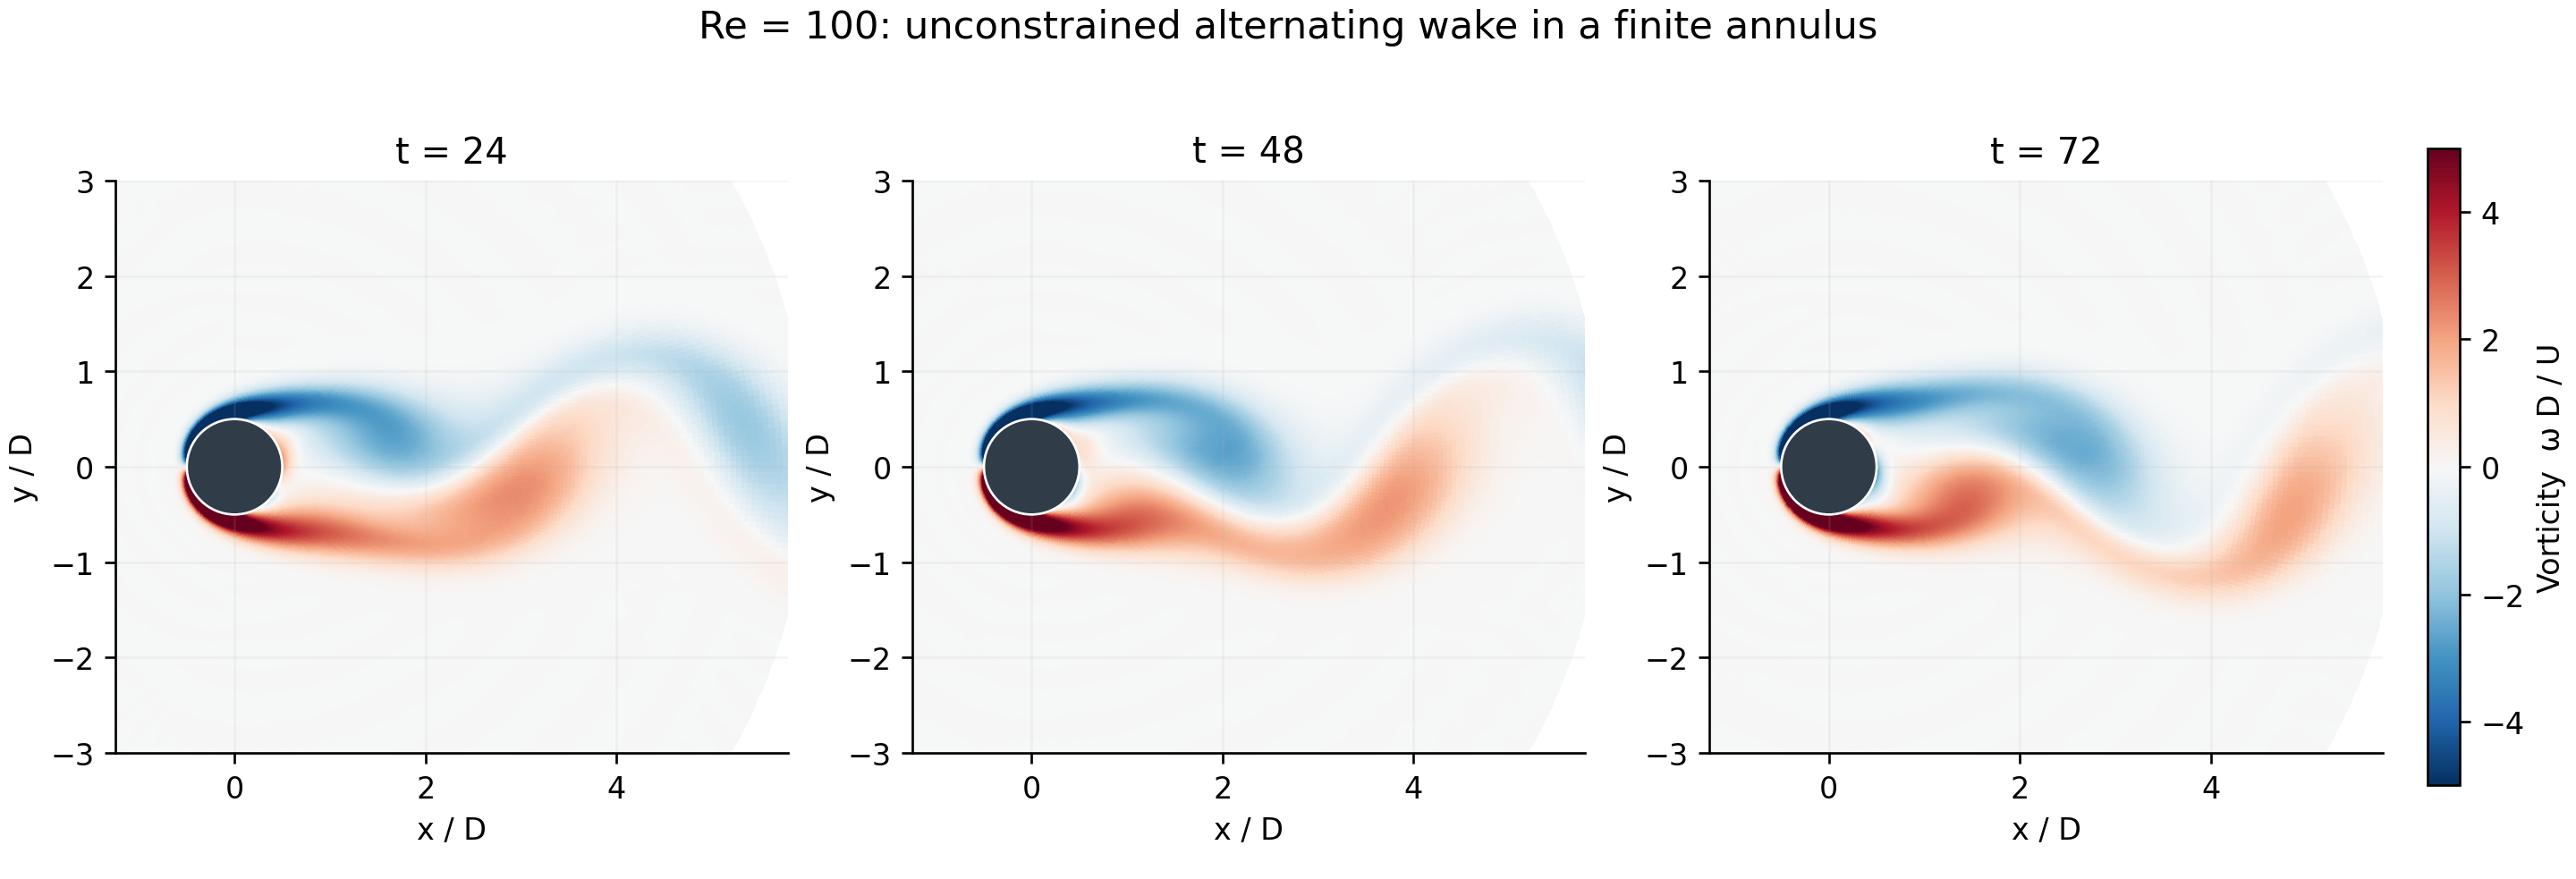
\includegraphics[width=\linewidth]{figures/finite_annulus_vorticity.png}
\caption{一条合格RFM41轨迹在 $t=24,48,72$ 的涡量，未施加反射对称约束。各图采用共同色标并展示圆环的局部视窗；完整外半径为6。}
\label{fig:annulus-wake}
\end{figure}

\begin{figure}[tbp]
\centering
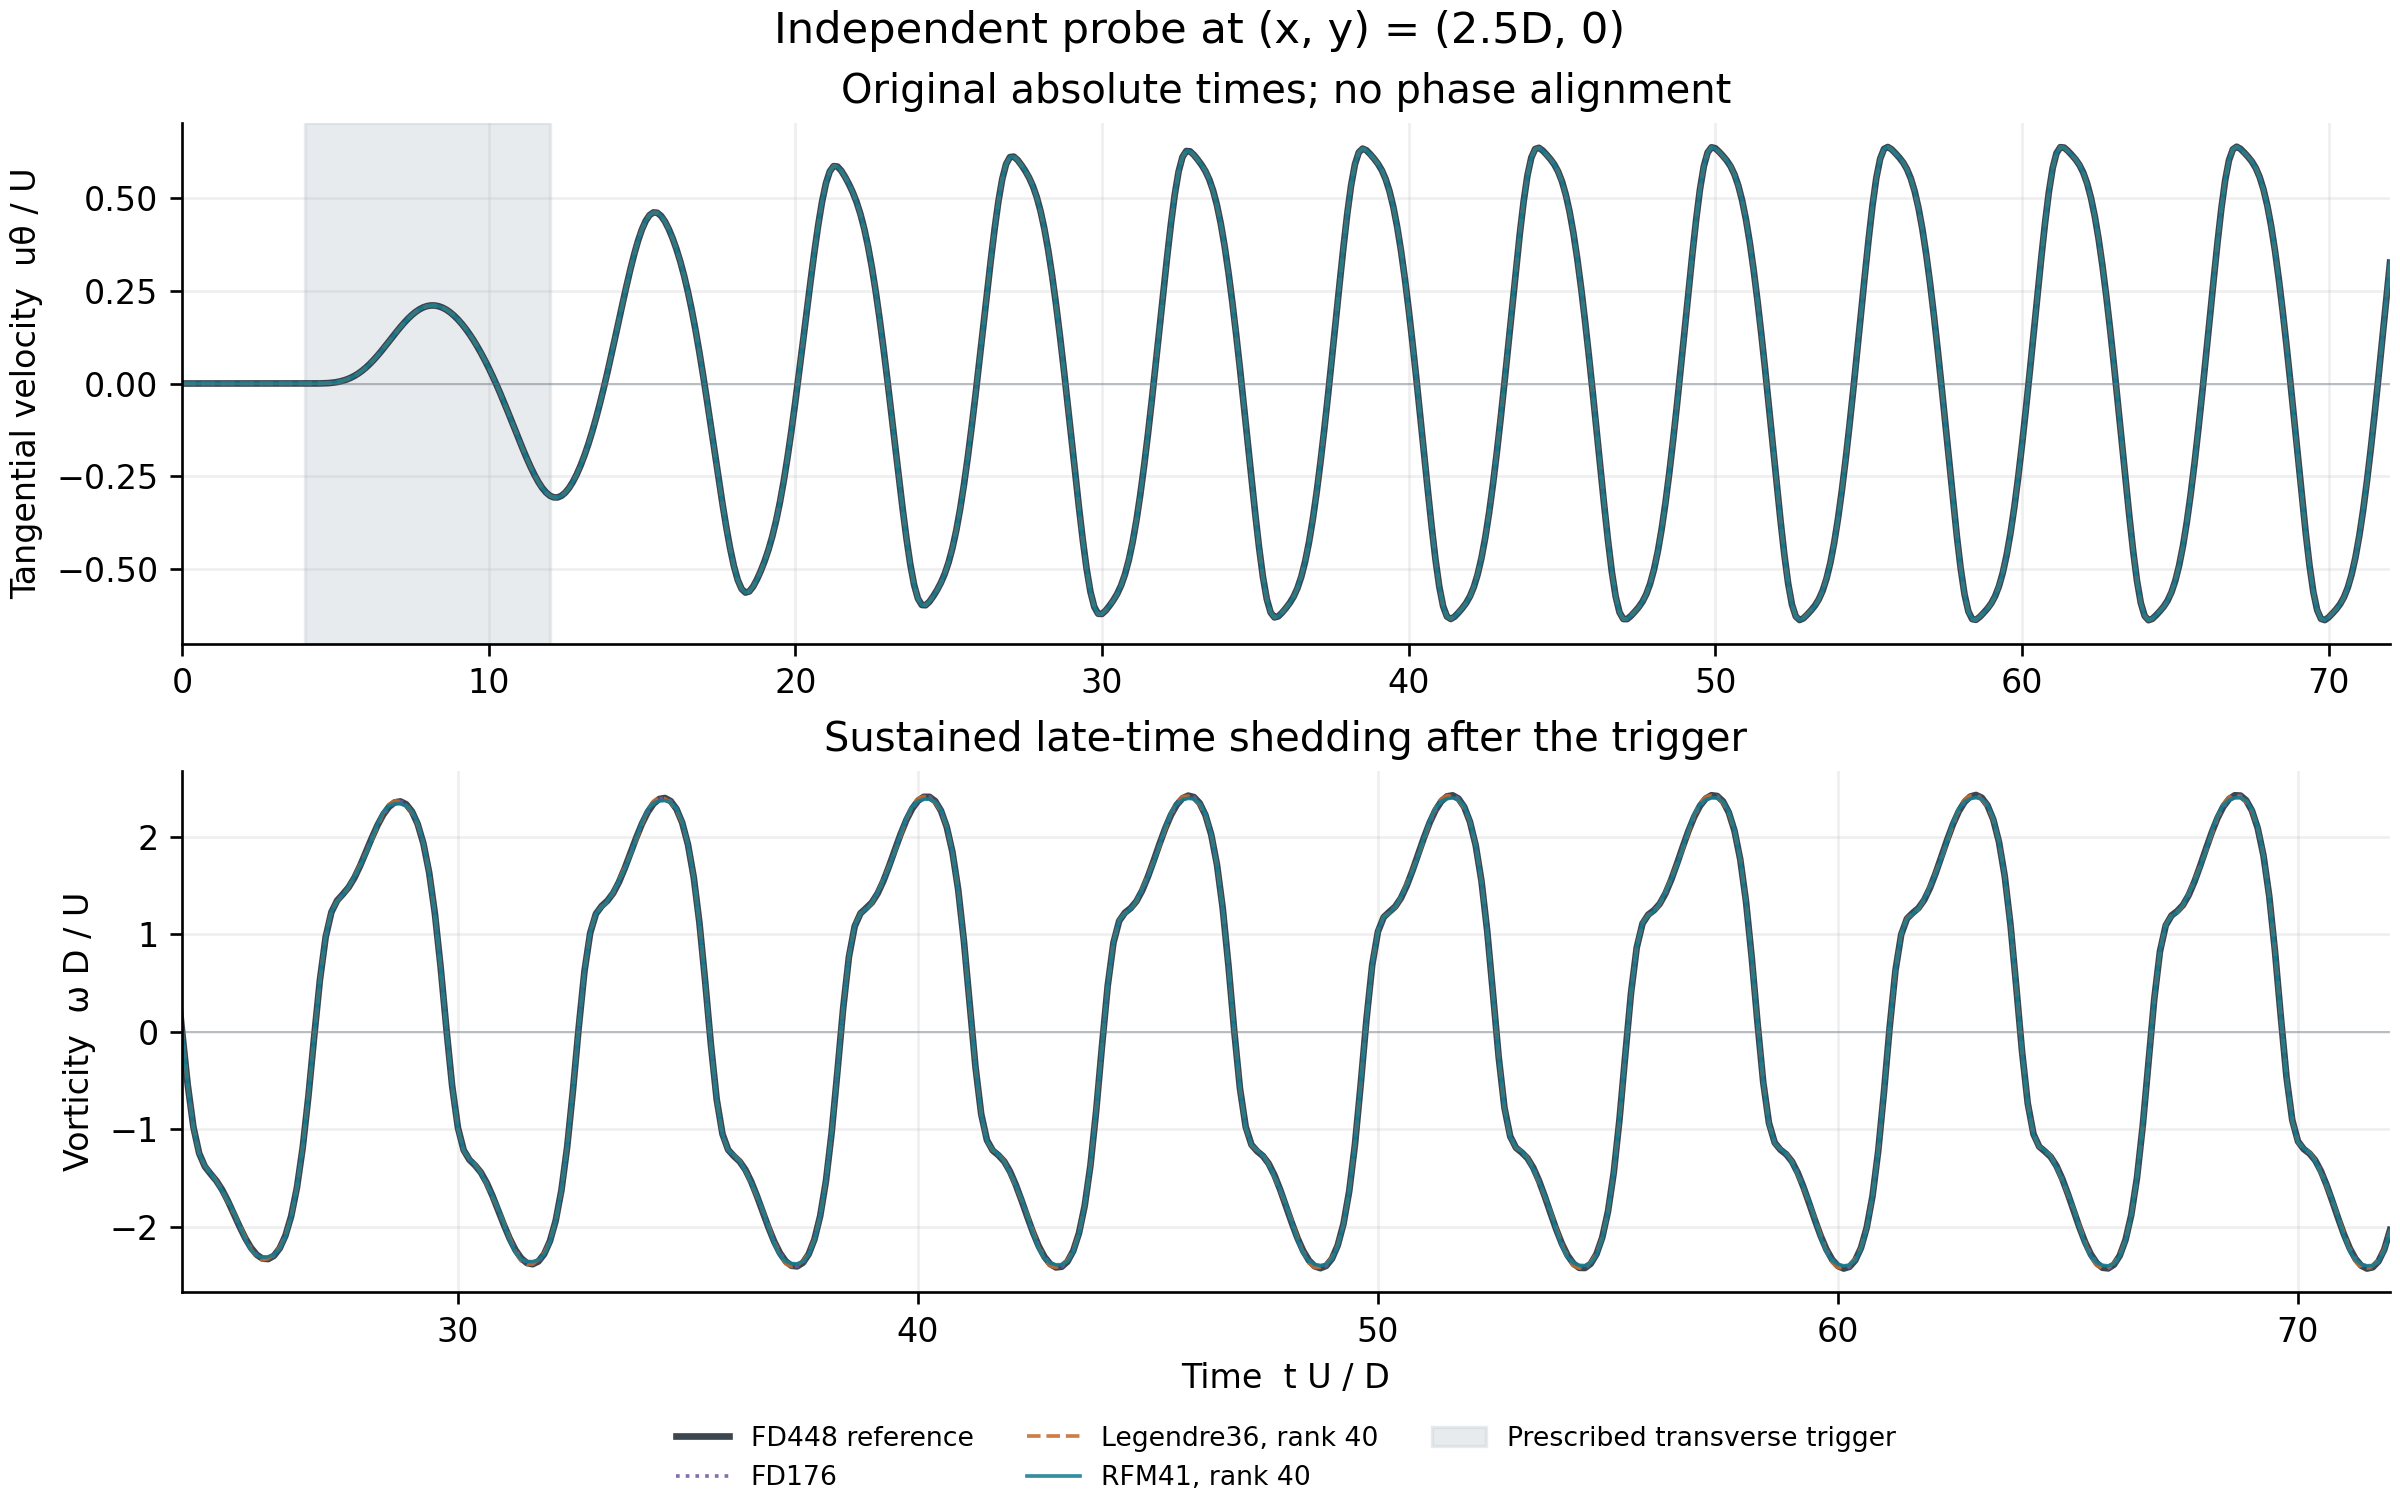
\includegraphics[width=0.88\linewidth]{figures/unshifted_wake_probes.png}
\caption{$x=2.5D,y=0$ 处未对齐探针。触发脉冲结束后仍持续交替脱落。RFM41和FD176来自合格GPU轨迹，Legendre36来自相应CPU资格，FD448为参考。}
\label{fig:wake-probes}
\end{figure}

\begin{table}[tbp]
\centering\small
\caption{两种分段方案的实际非线性求值次数，均在 $t=8$ 切换并推进至 $T=72$。}
\label{tab:workload}
\begin{tabularx}{\linewidth}{@{}Xrrr@{}}
\toprule
时间率 & 恒步 & 分段 & 减少量 \\
\midrule
$128\to112$ & 9,215 & 8,191 & 1,024（$11.11\%$） \\
$152\to136$ & 10,943 & 9,919 & 1,024（$9.36\%$） \\
\bottomrule
\end{tabularx}
\end{table}

表~\ref{tab:workload}直接读取运行时计数，而非根据名义阶数推断。后64个时间单位的时间率下降16，减少1,024步，实际非线性计数恰好相差同样数量。该收益对RFM与Legendre均成立。本文降秩时没有同步降低 $q$ 或角向FFT长度，因此不会额外减少一次非线性评估内部的FFT。工作量减少是算法层面的收益，能转化多少完整时间收益还取决于准备、线性代数、观测和运行时成本。

\section{算子性能与完整求解成本}
\label{sec:performance-results}

\subsection{FFT融合：局部有效与首次使用开销}

\begin{table}[tbp]
\centering\small
\caption{固定状态的CUDA图事件计时，单位为每次非线性评估的微秒。每配置为9个样本、每样本64次评估。比值仅适用于此局部测量。}
\label{tab:fusion-events}
\begin{tabularx}{\linewidth}{@{}Xrrr@{}}
\toprule
配置 & 原cuFFT & 融合实现 & 局部比值 \\
\midrule
Galerkin $N=225,q=66$ & 42.12 & 22.64 & 1.86 \\
Galerkin $N=243,q=76$ & 40.32 & 25.48 & 1.58 \\
FD176，$N=243$ & 85.13 & 61.00 & 1.40 \\
FD184，$N=243$ & 90.35 & 69.38 & 1.30 \\
\bottomrule
\end{tabularx}
\end{table}

表~\ref{tab:fusion-events}在固定状态和热输入数组下重复测量，不包括模型构造、编译、模块加载、FFT计划和物理轨迹推进。融合实现改善了四种被测非线性算子，其中较小Galerkin批的优势最大。该表不能推出任意FFT长度、设备或变换类型上都优于cuFFT；它比较的是输出定义一致的完整非线性流程，不是自定义单个FFT与无关库调用。

随后8条 $T=9$ 轨迹均通过参考与实现检查。相对同一warp观测的cuFFT路径，最大场差约 $1.78\times10^{-9}$；相对独立CPU轨迹约 $2.26\times10^{-7}$。推进时间缩短 $9\%$--$17\%$，但首次完整求解增加 $23\%$--$69\%$。编译与模块加载增加约0.25--0.62秒，而推进仅节省0.017--0.030秒。图~\ref{fig:fusion-cost}展示了这一反转，避免将重叠计时分项相加。

\begin{figure}[tbp]
\centering
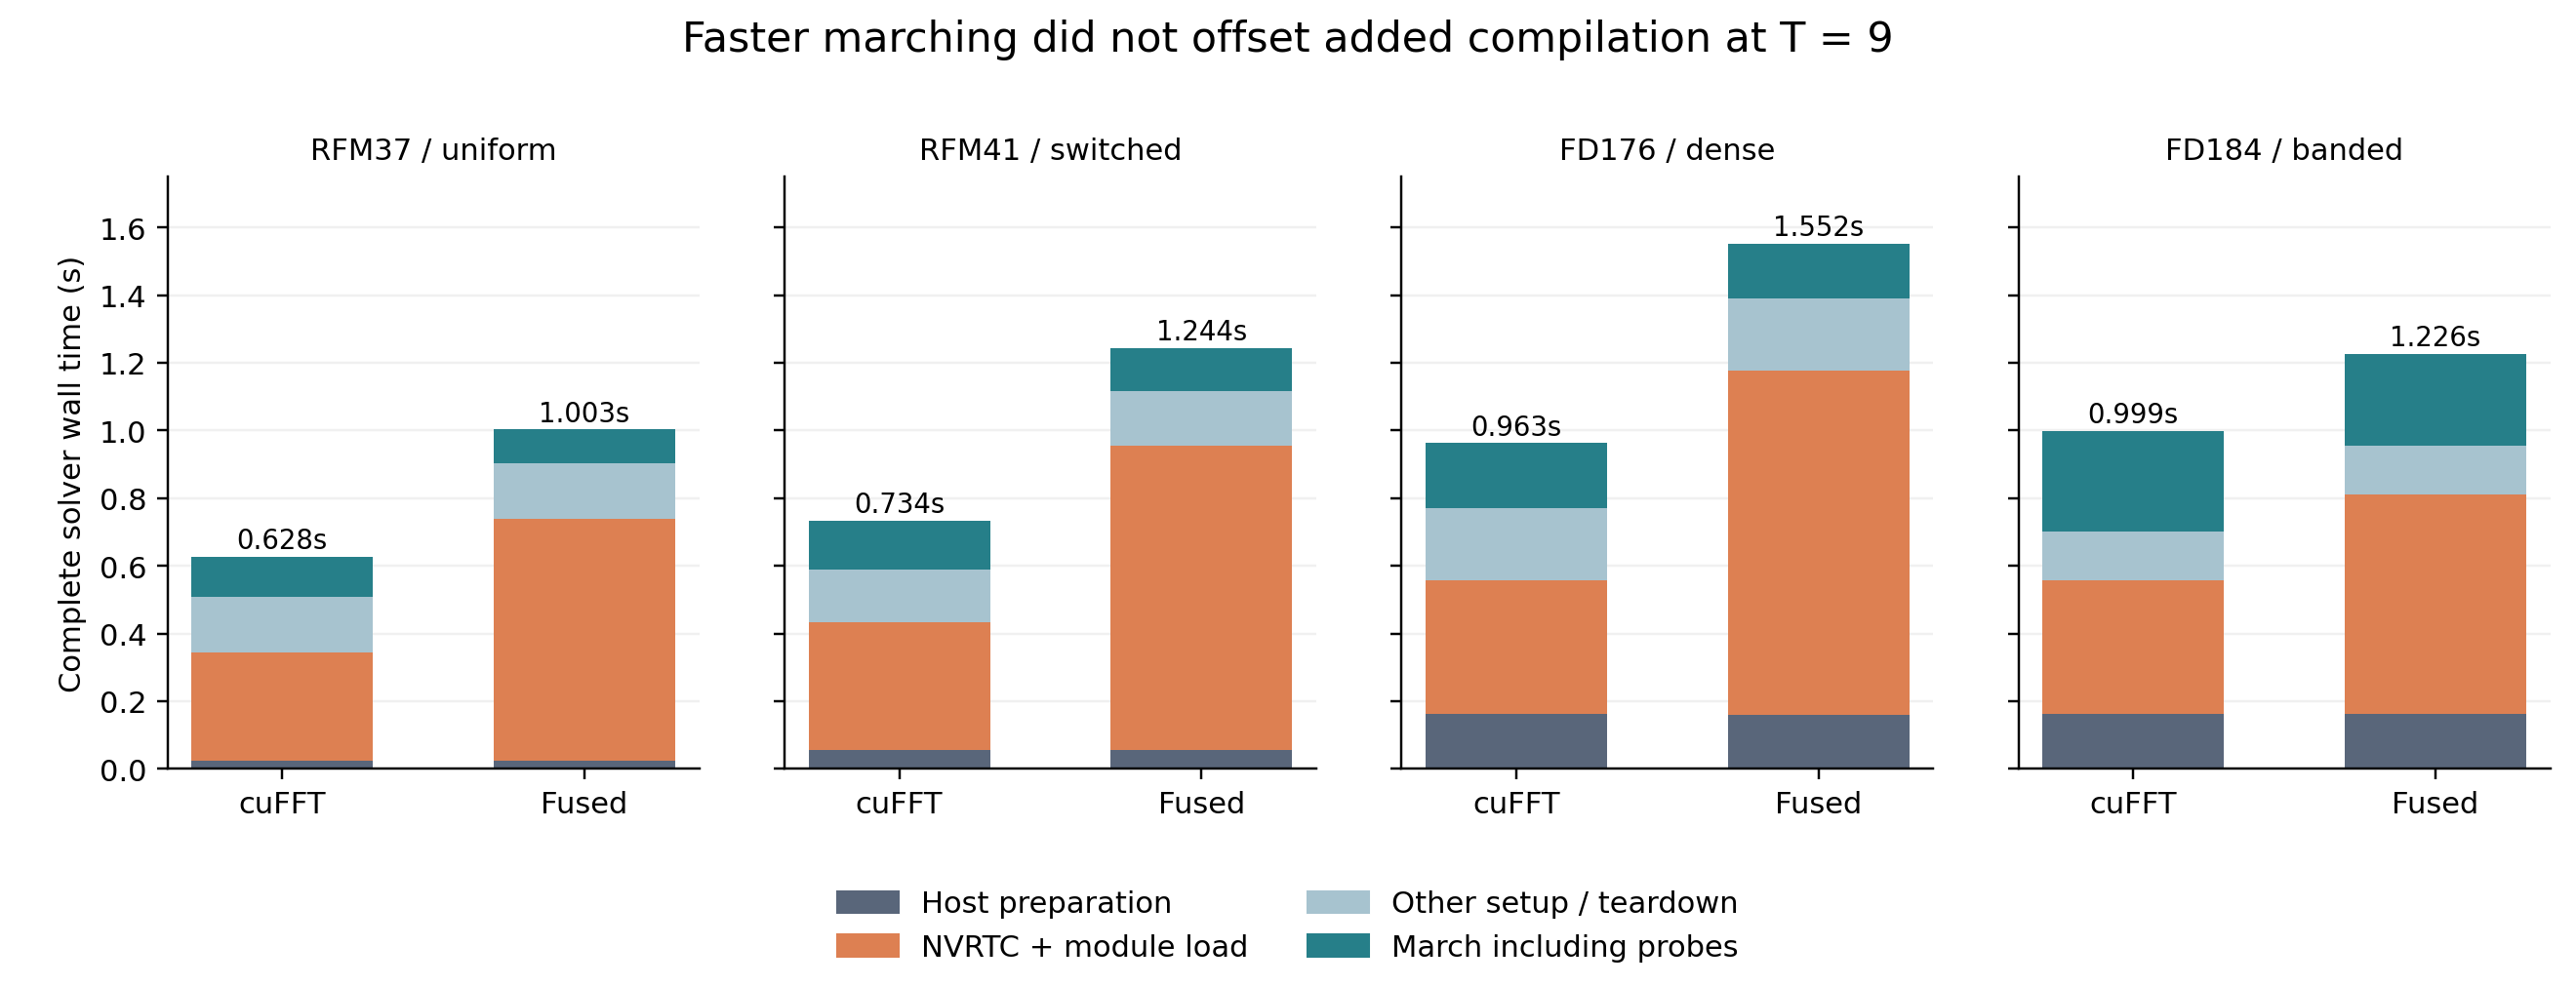
\includegraphics[width=\linewidth]{figures/t9_fusion_cost_breakdown.png}
\caption{顺序执行的 $T=9$ 融合诊断成本分解。编译与加载从其余运行时初始化中分离。该图定位首次使用代价，不提供尚缺失的最终 $T=72$ 排名。}
\label{fig:fusion-cost}
\end{figure}

缓存会改变这种权衡，但不取消晋升要求。后续严格命中诊断中，四组完整求解时钟均改善，新进程时钟却仅两组改善，因此未满足登记的晋升规则，最终 $T=72$ 群体仍采用原非线性FFT路径。这是工程筛选失败，不是短轨迹数值验证失败。把局部比值直接外推到长轨迹会忽略固定开销及各类工作所占比例的变化。

\subsection{观测核与共同实现收益}

warp归约改善的是另一部分流水线。固定状态的仅探针节点，Galerkin被测路径从约117--147微秒降至6--7微秒；FD176从727.5降至26.2微秒，FD184从760.3降至28.3微秒，局部比值约19--27。五条完整 $T=72$ 检查的保存状态和时刻逐位一致，改变求和顺序后完整探针最大相对差为 $9.26\times10^{-14}$。该算子不改变演化方程。

由于旧FD观测节点更贵，只给Galerkin应用此优化会扭曲比较。最终相关方法均使用warp观测。将热核节省量乘以观测次数可用于估计瓶颈位置，但不能替代修改后求解器的完整配对计时，更不能把局部19--27倍写成求解器整体倍率。

\subsection{缓存、启动与摊销条件}

显式缓存只保存项目核编译得到的PTX，不保存解、空间矩阵、CUDA上下文或cuFFT计划。键绑定源码、选项、目标架构、入口、编译器及依赖哈希。严格命中政策遇到缺失或损坏直接失败，不允许回退编译；\texttt{empty\_first}为每槽使用新目录，并计入编译、原子写入、读回验真与加载。驱动和操作系统缓存保持自然状态。因此“首次使用”是明确的缓存政策，不代表整台计算机已经重置为冷态。

三个stock PTX键合计147,782字节。三次新进程完整安装分别为2.7292、2.6392、2.6487秒，中位2.6487秒。只报告约0.93秒的NVRTC子阶段会遗漏大部分安装路径。若完整安装成本为 $C$、后续命中单次成本为 $H$、其它条件相同的首次使用成本为 $F$，则
\begin{equation}
\label{eq:cache-amortization}
 T_{\rm cache}(n)=C+nH,\qquad T_{\rm first}(n)=nF.
\end{equation}
存在交叉点需要 $F>H$ 且 $n>C/(F-H)$。最终批次没有提供已接受的 $F-H$ 配对估计，因此本文不给出实测盈亏平衡求解次数。该安装覆盖三个键，仅需其中一个键时的最小安装成本本轮未测。

早期50条高档批次通过其采样隔离检查，导入精简后，恒步与分段RFM的新进程配对中位加速比分别为1.293、1.301，而求解时钟比值接近1。这支持当时配置的启动改进，不能替代后续更强Legendre、共同warp观测和显式缓存政策的比较。混合这些历史行会混入不同实验处理。

\section{被淘汰候选与局部理论的边界}
\label{sec:negative-results}

\subsection{共同相位坐标与稠密输出布局}

共同相位基原型改善了局部线性代数诊断，但在现有稠密设备接口下，三相位准备时间增加约 $37\%$--$58\%$，实测见表~\ref{tab:phase-setup}。由于仍生成物理坐标下的稠密算子，设备存储仍为11.69--16.30 MB。实现需要支付特征分解与宽右端回变换，而非始终在对角坐标中完成计算。

\begin{table}[tbp]
\centering\small
\caption{局部相位准备计时，单位为毫秒。使用原型原锚点，不是后来推导的几何锚点。}
\label{tab:phase-setup}
\begin{tabularx}{\linewidth}{@{}Xrrr@{}}
\toprule
配置 & 原实现 & 直接三角求解 & 共同相位基 \\
\midrule
中档RFM & 34.27 & 47.41 & 51.96 \\
中档Legendre & 34.81 & 44.72 & 47.73 \\
高档RFM & 38.75 & 56.39 & 61.39 \\
高档Legendre & 45.71 & 62.00 & 66.22 \\
\bottomrule
\end{tabularx}
\end{table}

式~\eqref{eq:anchor}的解析锚点最小化条件数上界，尚未作为新的生产候选计时。变换后条件性更好、分解次数更少、存储更小与完整运行更快是四个不同命题。若后续保持共同坐标状态，需同时修改重构、提升、投影、观测，并重新验证浮点行为和完整轨迹；当前原型没有检验这种架构。

\subsection{能量结构不能保证粗步精度}

Lamb--BDF2候选冻结外推涡量，再迭代求解所得速度系统。附录~\ref{sec:app-lamb}给出离散反对称性与恒步能量恒等式，保留边界及代数残差做功。这些性质仅适用于所述离散更新与范数，不能消除涡量外推误差，也不能保证任意大步长下的精度。

在 $T=16$、时间率128下，RFM37和Legendre37的最坏涡量误差分别为 $0.364950\%$、$0.364784\%$，通过 $0.5\%$ 门槛；时间率64下分别升至约 $161.024\%$、$161.664\%$。首个保存的失败状态出现在 $t=4$，早于横向触发。检查点原方程残差仍不超过 $7.590\times10^{-10}$，做功修正后的能量缺陷不超过 $2.25\times10^{-15}$。因此线性系统解得很准、能量账闭合，与流场轨迹严重失真并不矛盾。

合格的时间率128候选所需一维FFT约为同空间显式控制的5.03倍。工作计数包含迭代及残差检查需要的乘积，单看名义步数会掩盖这些成本。时间率64方案同样需要更多变换且精度失败，因此该分支在进入 $T=72$ GPU比较之前被淘汰。

\subsection{稀疏非线性求值与图调度调整}

隔步计算真实非线性并作历史外推，在名义上能减少求值。相应标量测试的观测收敛阶为1.998--2.016，但修正后的NS试验在 $t=8$ 后启用此策略，分别在约 $t=9.508$、9.559溢出，普通控制则完成。失败轨迹不能提供有效精度或速度结果。这说明局部一致性与标量稳定性探针只能用于筛选，不能替代受驱动、模态耦合离散系统的验证。

两项实现试验数值正确，却未达到性能晋升要求。交替复用现有两个频谱历史缓冲，八对短轨迹逐位一致，但图模式两组配对中位推进差分别为 $-0.030$、$+0.018$ 毫秒，方向不稳定。将CUDA图块从24步改为48、64、128步，36条完整轨迹逐位一致；48步虽使计划图启动数减半，却没有替代方案同时通过预设推进、求解与新进程收益门槛。这些诊断没有完整外载隔离，不能支持微小而稳定的速度差，最终保留24步图块。

\section{最终完整计时的处置}
\label{sec:timing-disposition}

最终设计登记160槽，覆盖五个配对区块、两种缓存政策和合格方法。RFM种子按区块指定，确定性方法保持固定；实际优势需要完整求解与新进程两种时钟共同支持，后者还计入声明的监督及进程启动成本。每窗须完成预设顺序、数值验收及采样隔离，不允许针对失败槽选择性补上更干净的运行。

\begin{table}[tbp]
\centering\small
\caption{最终计时尝试与可接受解释。没有一项构成已接受的最终配对速度排名。}
\label{tab:timing-status}
\begin{tabularx}{\linewidth}{@{}p{0.22\linewidth}XX@{}}
\toprule
尝试 & 实际记录 & 对结论的影响 \\
\midrule
原始设计 & 完成两槽，第三槽未确认及时终止 & 配对区块不完整 \\
第一次恢复 & 预检出现外部活动，零槽启动 & 计时前拒绝该窗 \\
最终恢复 & 尝试12槽，11槽原始成功，第12槽终态发布失败 & 未通过完整性要求 \\
独立负载检查 & 最终活动区间外部CPU超过登记预算 & 独立违反隔离条件 \\
数值读回 & 12份保存轨迹均与资格数组一致，余148槽未尝试 & 保留数值证据，不生成排名 \\
\bottomrule
\end{tabularx}
\end{table}

最后一槽的求解器写出数值结果且精确进程状态成功退出，但随后权限错误阻止终态发布。现有记录不能识别原始锁持有者；后续纯CPU试验在受控读者配置下复现了文件发布失败，仍未证明它就是先前事件的原因。负载监测还独立记录到外部CPU活动超过每10秒0.2 CPU秒的预算。因此即使修复终态发布，也不能使这批历史记录变为合格隔离计时。

隔离机制采用采样进程身份和GPU预检，不是操作系统强制独占。短进程可能完全落在采样间隙，非研究应用的覆盖也有限。这些局限同样适用于通过采样检查的历史批次；对最终窗口而言，已记录的违规本身已足以拒绝计时，无需推断还存在何种未观测活动。

本文不从11条原始成功记录、资格阶段耗时或拼接旧两槽与恢复记录中构造最终加速比、置信区间和方法排序。高档窗口未完成，也使跨分辨率稳定性缺乏证据。结论是性能顺序未确定，而不是实测证明RFM胜出或败给最强传统对照。

\section{讨论与结论}
\label{sec:discussion}

现有证据能够区分数值设计与实现贡献。分段时间率减少实际非线性求值，对RFM与Legendre共同有效；两族均存在紧凑合格空间。自有融合核降低局部非线性代价，warp归约消除Galerkin与FD共同的观测瓶颈，启动精简和显式缓存改变另外的成本项。任何单项都不足以证明随机特征带来的完整速度优势。

最直接的已测瓶颈是短GPU工作负载与准备成本不匹配。历史剖析中主机空间准备约0.058秒，占约1.70秒完整求解的3.4\%。这只是特定配置诊断，不是普适上限，但不足以支持整套更换语言。重写已测热循环可能有效；只更换上层编排语言不会减少非线性求值次数、库FFT或设备矩阵工作。高层流动求解器也可以结合高效内核与数值库\cite{r14}。

有限外边界是主要物理局限。将 $R$ 从6增至8后，在共同 $r\leq4$ 区域，未对齐最大涡量差约50.39\%，其中包含累计相位影响。这是有限域模拟之间的敏感性结果，不是对连续真解误差的严格估计，因而不能把本次 $0.5\%$ 资格解释为无限外域圆柱绕流验证。本文亦未验证压力、升阻力、三维湍流、更高Re数或跨设备稳定速度优势。

本阶段没有在相同完整场、探针和计时协议下测量先进训练式PINN，因此本文比较的是固定特征Galerkin离散及其确定性和FD控制，不能对PINN训练方法作速度排序。前期方腔及其它流动研究也不能自动继承最终圆环资格；更宽的结论需要相应算例的参考与计时证据。

\label{sec:conclusion}
对于指定 $\mathrm{Re}=100$ 有限圆环问题，78条登记GPU资格轨迹全部通过共同速度与涡量门槛。两种分段策略将非线性求值减少 $11.11\%$、$9.36\%$。融合FFT在局部与短程推进有效，却在首次完整成本上失去优势；更激进的非线性更新候选未通过精度或工作量要求。最终隔离批次未被接受，因此尚未建立相对优化Legendre和四阶空间FD的稳定完整求解优势。可支持的贡献是数学适配、底层核实现，以及依据证据区分这些影响的归因分析。

\section*{数据与代码可用性}

NS实验对应归档修订
\href{https://github.com/LStar404/rfm-navier-stokes-research/tree/6f2b3500964d3d5153b8400018236c4702ef94f8}{\texttt{6f2b350}}。
归档保留源码、协议、配置身份、资格评分、成功记录和失败尝试。仓库目前限制访问，公开独立复现仍需要可访问的发布版本。附录~\ref{sec:app-evidence}将归档NS表图映射到原始记录。修订稿新增的独立算子示例及正确性检查另作标记，它们不为冻结的NS证据增加新的PDE轨迹、性能测量或已接受的隔离计时批次。

\FloatBarrier
\bibliography{references}
\appendix
\section{符号、误差网格与复现顺序}\label{sec:app-setup}

模型、边界提升、特征变换与弱式的完整定义见第\ref{sec:space-discretization}节及第\ref{sec:numerical-method}节。这里集中给出跨章节符号和不参与求解的误差重构网格，避免把输入特征数、实际秩、求积数和 FFT 长度混为同一分辨率。

\begin{table}[!htbp]
\centering\small
\caption{主要符号及其计算含义}
\begin{tabularx}{\linewidth}{@{}lX@{}}
\toprule
符号 & 含义 \\
\midrule
$s,z,L$ & $s=\log(r/a)$，$L=\log(R/a)$，$z=s/L$ \\
$m,d,d_0$ & 输入径向特征数、实际非零模保留秩、独立均值秩（30） \\
$K,N,q$ & 最大保留角模、角向 FFT 长度、Galerkin 径向求积节点数 \\
$n$ & FD 径向区间数；节点 $n+1$、内部未知数 $n-1$ \\
$M_k,K_k$ & 非零角模的质量矩阵和黏性矩阵 \\
$H,h,\rho$ & 桥接前后时间步及其比值 $h/H$ \\
$H_{\rm ref}$ & 如用作相位白化矩阵，表示 $a_{\rm ref}M+h_{\rm ref}K$；正文亦记 $H$ \\
$N_{\rm nl},C_{\rm nl}$ & 真实非线性求值次数及一次评估的有效成本 \\
\bottomrule
\end{tabularx}
\end{table}

\begin{table}[!htbp]
\centering\small
\caption{独立物理误差重构网格}
\label{tab:app-score-grids}
\begin{tabularx}{\linewidth}{@{}Xrrr@{}}
\toprule
网格 & 径向节点 & 角向节点 & 角向偏移参数 \\
\midrule
Gauss & 123 & 433 & 0.23 \\
等间隔中点 & 129 & 449 & 0.43 \\
分段层加密 & 144（96/24/24） & 457 & 0.31 \\
\bottomrule
\end{tabularx}
\end{table}

评价权包含 $r^2\,ds\,d\theta$，速度范数联合使用 $u_r,u_\theta$。19个物理误差检查时刻为0.5、1、2、4、6、8、8.125、8.5、9、10、12、16、24、36、48、54、60、66、72。分段方案另保存 $8+1/\mathrm{late\_rate}$ 和 $8+2/\mathrm{late\_rate}$ 两个状态用于实现一致性检查，不能将它们称为新增的双参考物理评分时刻。探针位于 $(x/D,y/D)=(1.5,0),(2.5,0),(3.5,0)$，按 $\Delta t=0.125$ 保存，含初始零值共577点；各点保存横向速度和涡量，共六条历史。

复现时先固定附录\ref{sec:app-evidence}中的归档身份、源文件和两份数值参考，再核对每个配置的几何、种子、保留秩、时间率和缓存政策。重构物理场后逐网格、逐时刻评分，检查同离散 CPU/GPU 一致性与分段三角保护。只有通过这些门槛的候选才能进入独立计时；数值资格批次中的并发耗时不能充当隔离计时。计时协议的完整性、终态记录与外部负载检查应先于速度比计算。最后另行运行修订版的独立算子样例，其合格标志仅覆盖合成固定状态，不替代以上流动验证。

\section{冻结涡量结构与适用范围}\label{sec:app-lamb}

\setcounter{equation}{0}
\renewcommand{\theequation}{B.\arabic{equation}}
\renewcommand{\theHequation}{appendix.B.\arabic{equation}}

在正确实 Fourier 权重下，均值权为1，非零模实虚部权各为2。固定涡量 \(\omega^*\) 的弱配对为 \(\sum_i w_i\omega_i^*(u_{\theta,i}v_{r,i}-u_{r,i}v_{\theta,i})\)。同一求积及互为伴随的重构和投影使交换 u、v 后变号，因此齐次离散矩阵 \(F^\top=-F\)。该结构需要离散检查，不能只从连续方程能量性质推定。

\begin{equation}
\label{eq:lamb-update}
[(3/2)M+hK-hF]x_{n+1}=2Mx_n-\tfrac12 Mx_{n-1}+L_{n+1}+R_{n+1}.
\end{equation}

L 含边界提升及外力，R 定义为原方程左端减去含 L 的原右端。定义加权半范数及 G 如下：

\begin{equation}
\label{eq:lamb-norm}
\|x\|_M^2=x^\top Mx,\qquad G(x,y)=\|x\|_M^2+\|2x-y\|_M^2.
\end{equation}

\(K\) 加权半范数同理。固定步长下将式~\eqref{eq:lamb-update} 与 \(4x_{n+1}\) 配对，得到

\begin{equation}
\label{eq:lamb-energy}
\begin{aligned}&G(x_{n+1},x_n)-G(x_n,x_{n-1})+\|x_{n+1}-2x_n+x_{n-1}\|_M^2+4h\|x_{n+1}\|_K^2\\&\qquad=4\langle x_{n+1},L_{n+1}\rangle+4\langle x_{n+1},R_{n+1}\rangle.\end{aligned}
\end{equation}

恒等式由 \(4\langle x,(3/2)Mx-2My+(1/2)Mz\rangle\) 展开得到，\(F\) 项抵消。\(R\) 已处于式~\eqref{eq:lamb-update} 的步长尺度，右侧残差做功不再乘 \(h\)。无外力、齐次边界且精确求解时，\(L=R=0\)，\(G\) 单调不增。驱动问题需要保留右端。\(G\) 衡量齐次速度部分的离散能量。

再令 \(A=(3/2)M+hK=LL^\top\)、\(S=L^{-1}FL^{-\top}\)，则 \(S^\top=-S\)。对称变换后的 \(B=I-hS\) 满足 \(B^\top B=BB^\top=I-h^2S^2\)，故对任意 z 有 \(\|Bz\|_2^2=\|z\|_2^2+h^2\|Sz\|_2^2\)，进而 \(\sigma_{\min}(B)\ge1\)。该保证只在变换坐标中成立，不保证 GMRES 次数、变换往返误差或物理精度改善。正文报告的粗步失败与增加的 FFT 工作量因此必须保留。

\section{主要证据与复核入口}\label{sec:app-evidence}

以下记录均对应固定提交6f2b350。标签链接直达原始文件。路径中的 v7、v8 表示实验版本而非独立论文结果。理论说明、数值资格、局部计时与完整批次的作用不同。

\noindent\href{https://github.com/LStar404/rfm-navier-stokes-research/blob/6f2b3500964d3d5153b8400018236c4702ef94f8/work/rfm_v6/full_case.py}{C1 算例与边界}\par\nopagebreak
{\small\nolinkurl{work/rfm_v6/full_case.py}}\par\smallskip

\noindent\href{https://github.com/LStar404/rfm-navier-stokes-research/blob/6f2b3500964d3d5153b8400018236c4702ef94f8/work/rfm_v6/full_galerkin.py}{C2 空间与矩阵}\par\nopagebreak
{\small\nolinkurl{work/rfm_v6/full_galerkin.py}}\par\smallskip

\noindent\href{https://github.com/LStar404/rfm-navier-stokes-research/blob/6f2b3500964d3d5153b8400018236c4702ef94f8/work/rfm_v7/theory_sbdf2_single_bridge.txt}{C3 桥接与提升推导}\par\nopagebreak
{\small\nolinkurl{work/rfm_v7/theory_sbdf2_single_bridge.txt}}\par\smallskip

\noindent\href{https://github.com/LStar404/rfm-navier-stokes-research/blob/6f2b3500964d3d5153b8400018236c4702ef94f8/work/rfm_v8/theory_phase_pencil_scope_note.txt}{C4 相位矩阵及锚点边界}\par\nopagebreak
{\small\nolinkurl{work/rfm_v8/theory_phase_pencil_scope_note.txt}}\par\smallskip

\noindent\href{https://github.com/LStar404/rfm-navier-stokes-research/blob/6f2b3500964d3d5153b8400018236c4702ef94f8/work/rfm_v8/galerkin_phase_pencil_audit_canonical_mean.json}{C5 相位准备实测}\par\nopagebreak
{\small\nolinkurl{work/rfm_v8/galerkin_phase_pencil_audit_canonical_mean.json}}\par\smallskip

\noindent\href{https://github.com/LStar404/rfm-navier-stokes-research/blob/6f2b3500964d3d5153b8400018236c4702ef94f8/work/rfm_v8/rank_fair_cache_qualification_output/protocol.json}{C6 最终39配置及双缓存协议}\par\nopagebreak
{\small\nolinkurl{work/rfm_v8/rank_fair_cache_qualification_output/protocol.json}}\par\smallskip

\noindent\href{https://github.com/LStar404/rfm-navier-stokes-research/blob/6f2b3500964d3d5153b8400018236c4702ef94f8/work/rfm_v8/rank_fair_cache_qualification_output/qualification_summary.json}{C7 最终78条数值资格}\par\nopagebreak
{\small\nolinkurl{work/rfm_v8/rank_fair_cache_qualification_output/qualification_summary.json}}\par\smallskip

\noindent\href{https://github.com/LStar404/rfm-navier-stokes-research/blob/6f2b3500964d3d5153b8400018236c4702ef94f8/work/rfm_v8/rank_parity_expansion_output/summary.json}{C8 秩扩展与失败候选}\par\nopagebreak
{\small\nolinkurl{work/rfm_v8/rank_parity_expansion_output/summary.json}}\par\smallskip

\noindent\href{https://github.com/LStar404/rfm-navier-stokes-research/blob/6f2b3500964d3d5153b8400018236c4702ef94f8/work/rfm_v8/fused_march_t9_output/summary.json}{C9 融合算子与短程总成本}\par\nopagebreak
{\small\nolinkurl{work/rfm_v8/fused_march_t9_output/summary.json}}\par\smallskip

\noindent\href{https://github.com/LStar404/rfm-navier-stokes-research/blob/6f2b3500964d3d5153b8400018236c4702ef94f8/work/rfm_v8/thin_formal_high_verification.json}{C10 历史启动改进隔离核验}\par\nopagebreak
{\small\nolinkurl{work/rfm_v8/thin_formal_high_verification.json}}\par\smallskip

\noindent\href{https://github.com/LStar404/rfm-navier-stokes-research/blob/6f2b3500964d3d5153b8400018236c4702ef94f8/work/rfm_v8/lamb_t16_qualification_output/summary.json}{C11 Lamb短程精度及工作量}\par\nopagebreak
{\small\nolinkurl{work/rfm_v8/lamb_t16_qualification_output/summary.json}}\par\smallskip

\noindent\href{https://github.com/LStar404/rfm-navier-stokes-research/blob/6f2b3500964d3d5153b8400018236c4702ef94f8/work/rfm_v8/rank_fair_cache_recovery_formal_final_closure/final_closure.json}{C12 最终完整计时结案}\par\nopagebreak
{\small\nolinkurl{work/rfm_v8/rank_fair_cache_recovery_formal_final_closure/final_closure.json}}\par\smallskip

表~\ref{tab:accuracy}由全部78份 independent\_score.json 逐组重算。表~\ref{tab:workload}计数取资格输出 slot\_000、slot\_010、slot\_026、slot\_036 的 result.json 中 metadata.nonlinear\_evaluations。表~\ref{tab:fusion-events}采用固定态图事件记录，表~\ref{tab:phase-setup}采用局部相位准备审计。图~\ref{fig:annulus-wake}、\ref{fig:wake-probes}与\ref{fig:fusion-cost}沿用同一归档内已核验的绘图与数据来源。所有速度解释均保留各自计时范围，不跨批次拼接为新的排名。

补充材料 \nolinkurl{supplement/evidence_revision.json} 记录归档来源哈希。前次修订的独立算子及实际GPU验证见 \nolinkurl{supplement/operator_sample/}；本次新增CPU实验及维护测试见第~\ref{sec:review-experiments}节与数据可用性说明。各目录README提供复现命令。

\end{document}
